% ============================================================
% BACKUP SLIDES
% ============================================================

\begin{frame}[plain]
    \centering
    \vfill

    {\LARGE\bfseries BACKUP SLIDES}

    \vfill
\end{frame}

% ============================================================
% NACA0012 -- HTC
% ============================================================

\begin{frame}{\small NACA0012 -- Convective Heat-Transfer Coefficient}
\scriptsize

\vspace{-0.15cm}

\begin{columns}[T,onlytextwidth]

% ------------------------------------------------------------
% AE3932
% ------------------------------------------------------------
\begin{column}{0.5\textwidth}
    \centering
    \textbf{AE3932}

    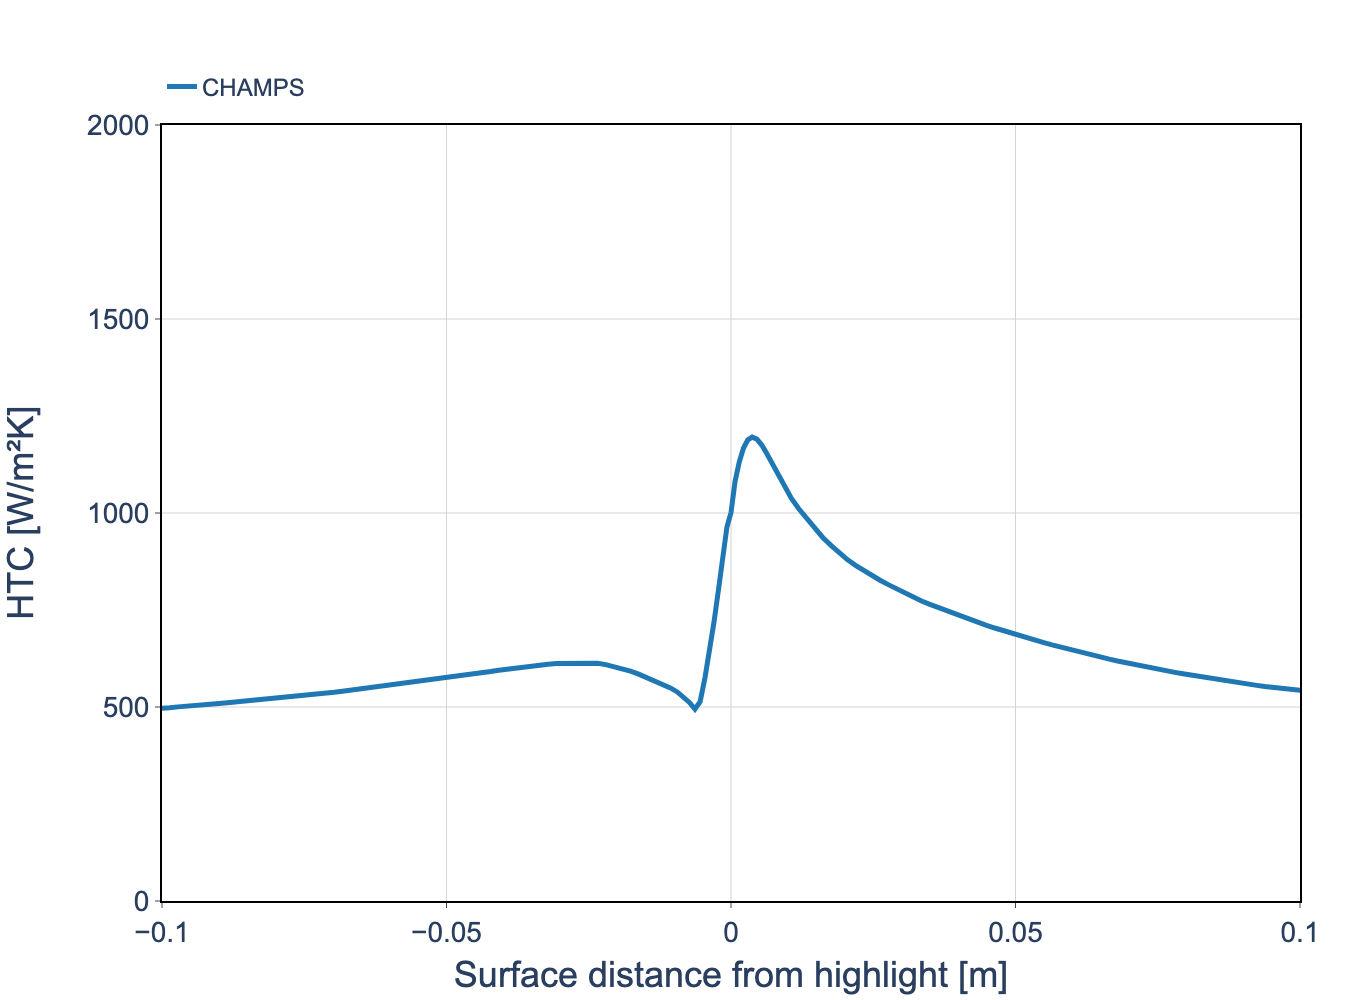
\includegraphics[
        width=\textwidth,
        trim={0cm 0cm 1cm 2.6cm},
        clip
    ]
    {FIGURES/NACA0012/HTC/tc_naca0012_ae3932_L1_htc_vs_s_slice_0p9144_all_roughness.png}
\end{column}

\hspace{-0.04\textwidth}

% ------------------------------------------------------------
% AE3933
% ------------------------------------------------------------
\begin{column}{0.5\textwidth}
    \centering
    \textbf{AE3933}
    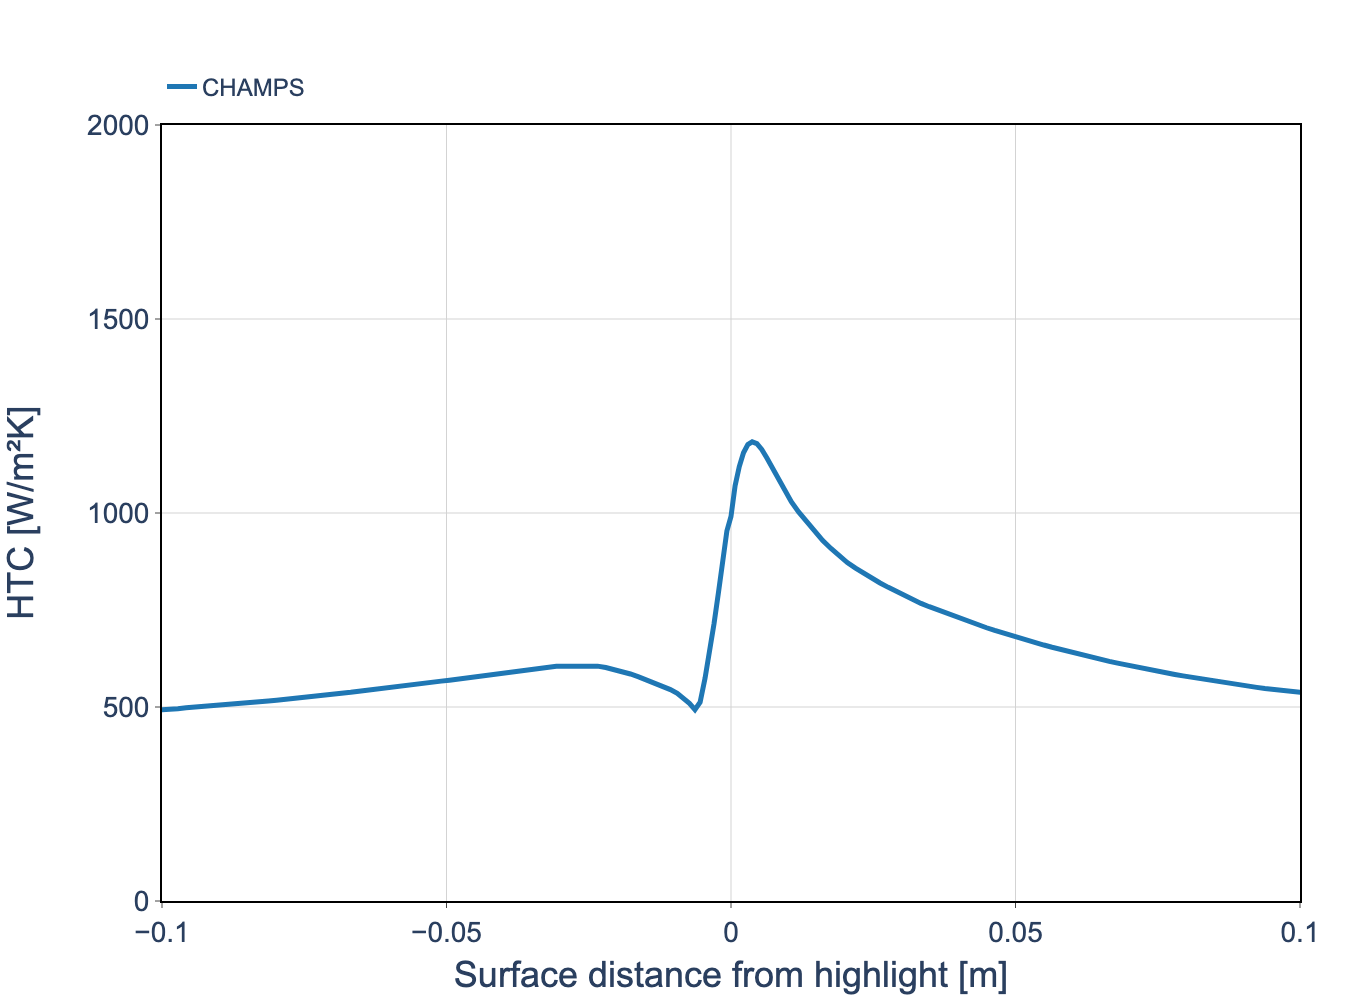
\includegraphics[
        width=\textwidth,
        trim={0cm 0cm 1cm 2.6cm},
        clip
    ]
    {FIGURES/NACA0012/HTC/tc_naca0012_ae3933_L1_htc_vs_s_slice_0p9144_all_roughness.png}
\end{column}

\end{columns}

\vspace{-0.15cm}

\end{frame}

% ============================================================
% BACKUP -- NACA0012 Freezing Fraction
% ============================================================

\begin{frame}{\small NACA0012 -- Freezing Fraction}
\scriptsize

\vspace{-0.15cm}

\begin{columns}[T,onlytextwidth]

% ------------------------------------------------------------
% AE3932
% ------------------------------------------------------------
\begin{column}{0.50\textwidth}
    \centering
    \textbf{AE3932}

    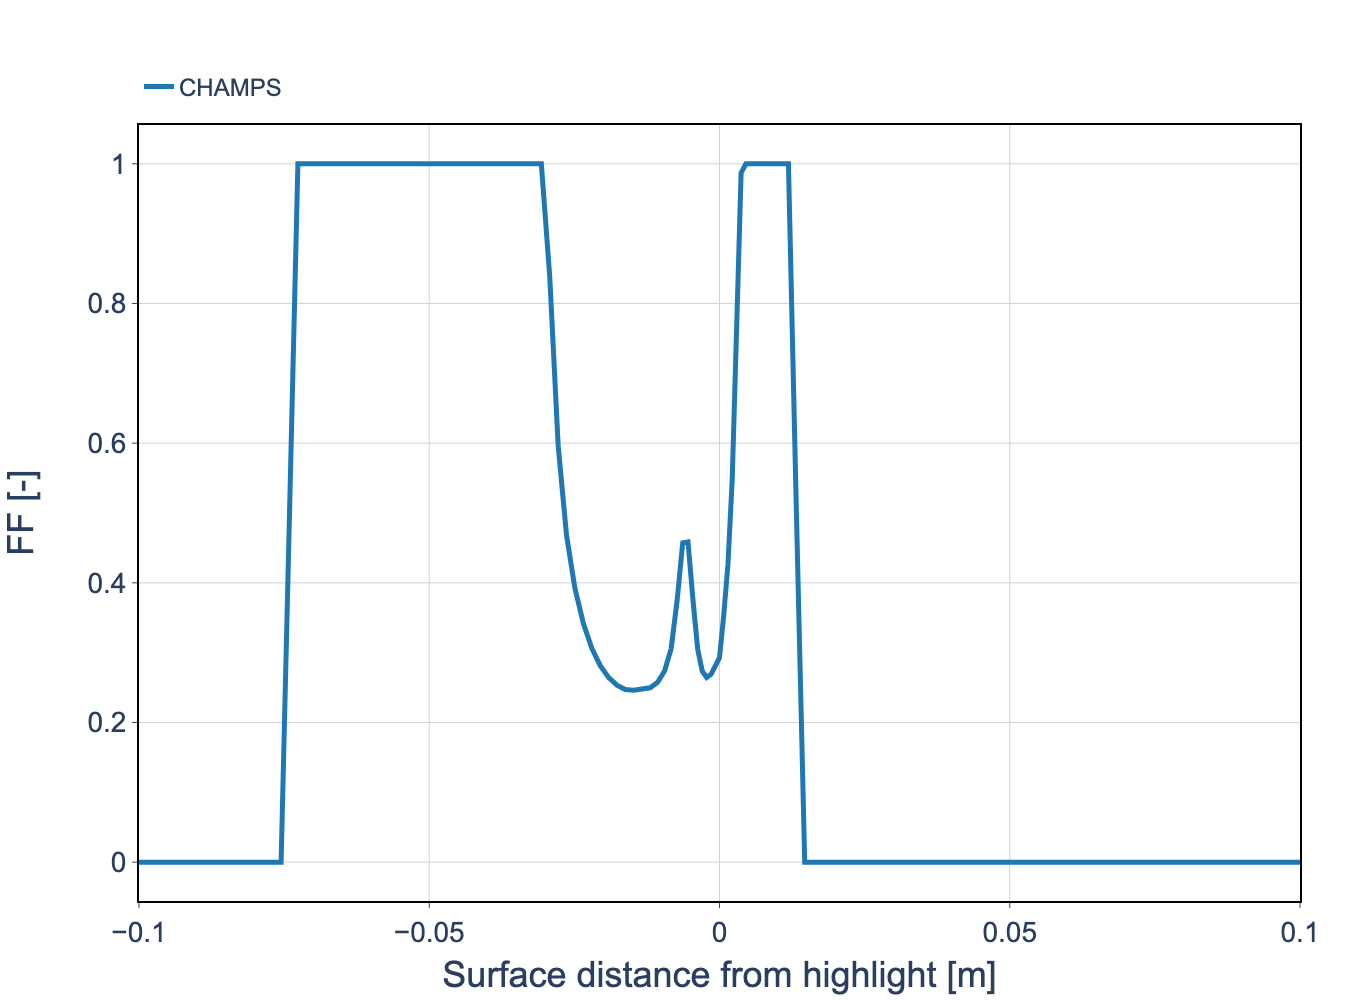
\includegraphics[
        width=\textwidth,
        trim={0cm 0cm 0cm 1.8cm},
        clip
    ]
    {FIGURES/NACA0012/SURF_TEMP_FF/tc_naca0012_ae3932_L1_freezing_fraction_vs_s_slice_0p9144_all_roughness.png}
\end{column}

% ------------------------------------------------------------
% AE3933
% ------------------------------------------------------------
\begin{column}{0.50\textwidth}
    \centering
    \textbf{AE3933}

    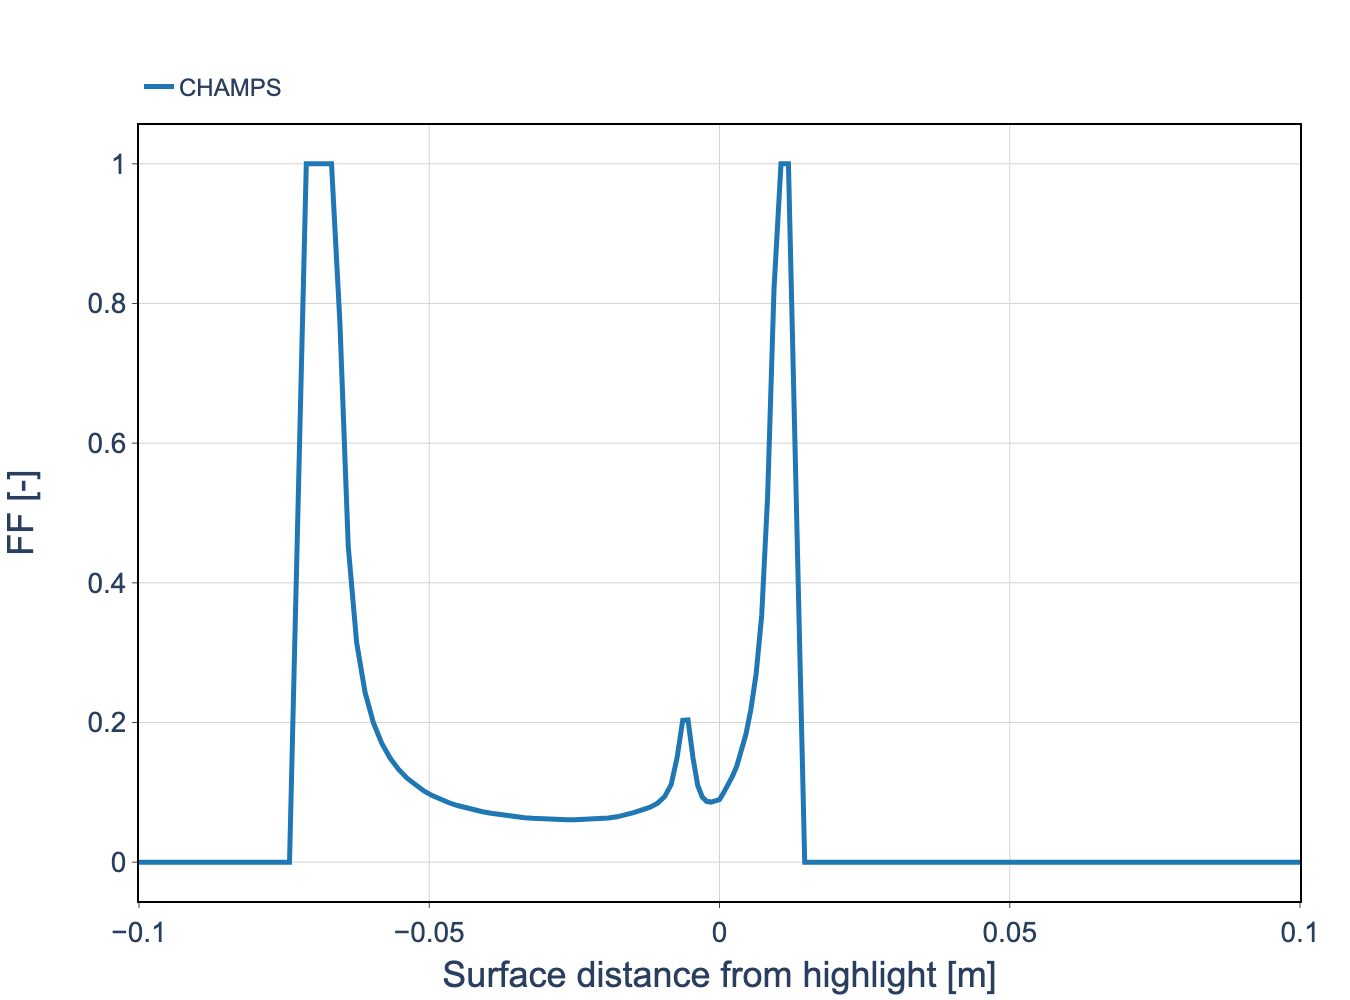
\includegraphics[
        width=\textwidth,
        trim={0cm 0cm 0cm 1.8cm},
        clip
    ]
    {FIGURES/NACA0012/SURF_TEMP_FF/tc_naca0012_ae3933_L1_freezing_fraction_vs_s_slice_0p9144_all_roughness.png}
\end{column}

\end{columns}

\end{frame}


% ============================================================
% BACKUP -- NACA0012 Surface Temperature
% ============================================================

\begin{frame}{\small NACA0012 -- Surface Temperature}
\scriptsize

\vspace{-0.15cm}

\begin{columns}[T,onlytextwidth]

% ------------------------------------------------------------
% AE3932
% ------------------------------------------------------------
\begin{column}{0.50\textwidth}
    \centering
    \textbf{AE3932}

    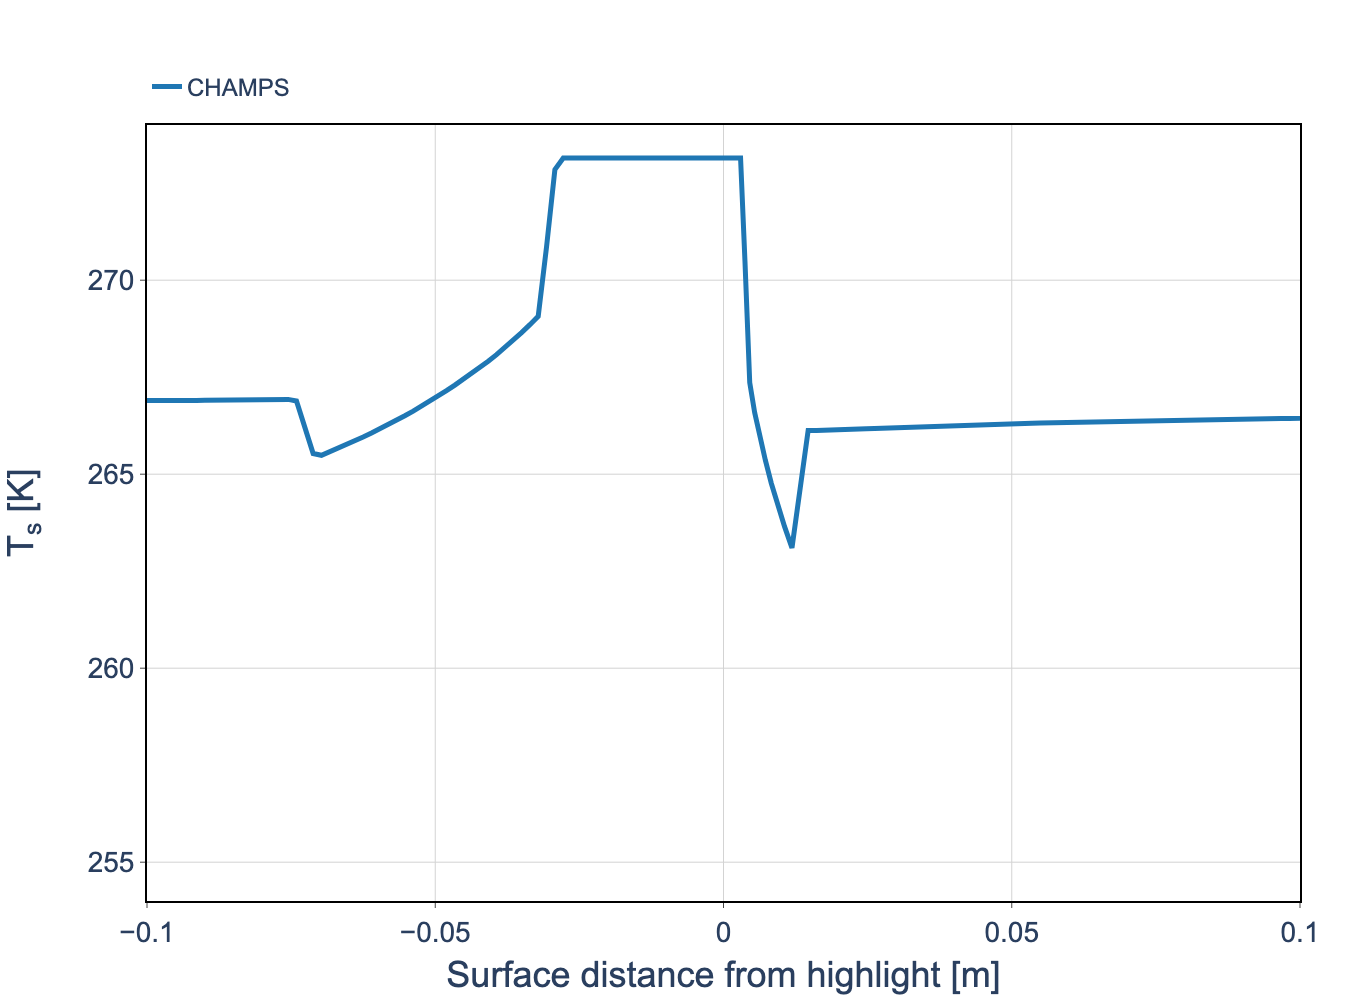
\includegraphics[
        width=\textwidth,
        trim={0cm 0cm 0cm 1.8cm},
        clip
    ]
    {FIGURES/NACA0012/SURF_TEMP_FF/tc_naca0012_ae3932_L1_surface_temperature_vs_s_slice_0p9144_all_roughness.png}
\end{column}

% ------------------------------------------------------------
% AE3933
% ------------------------------------------------------------
\begin{column}{0.50\textwidth}
    \centering
    \textbf{AE3933}

    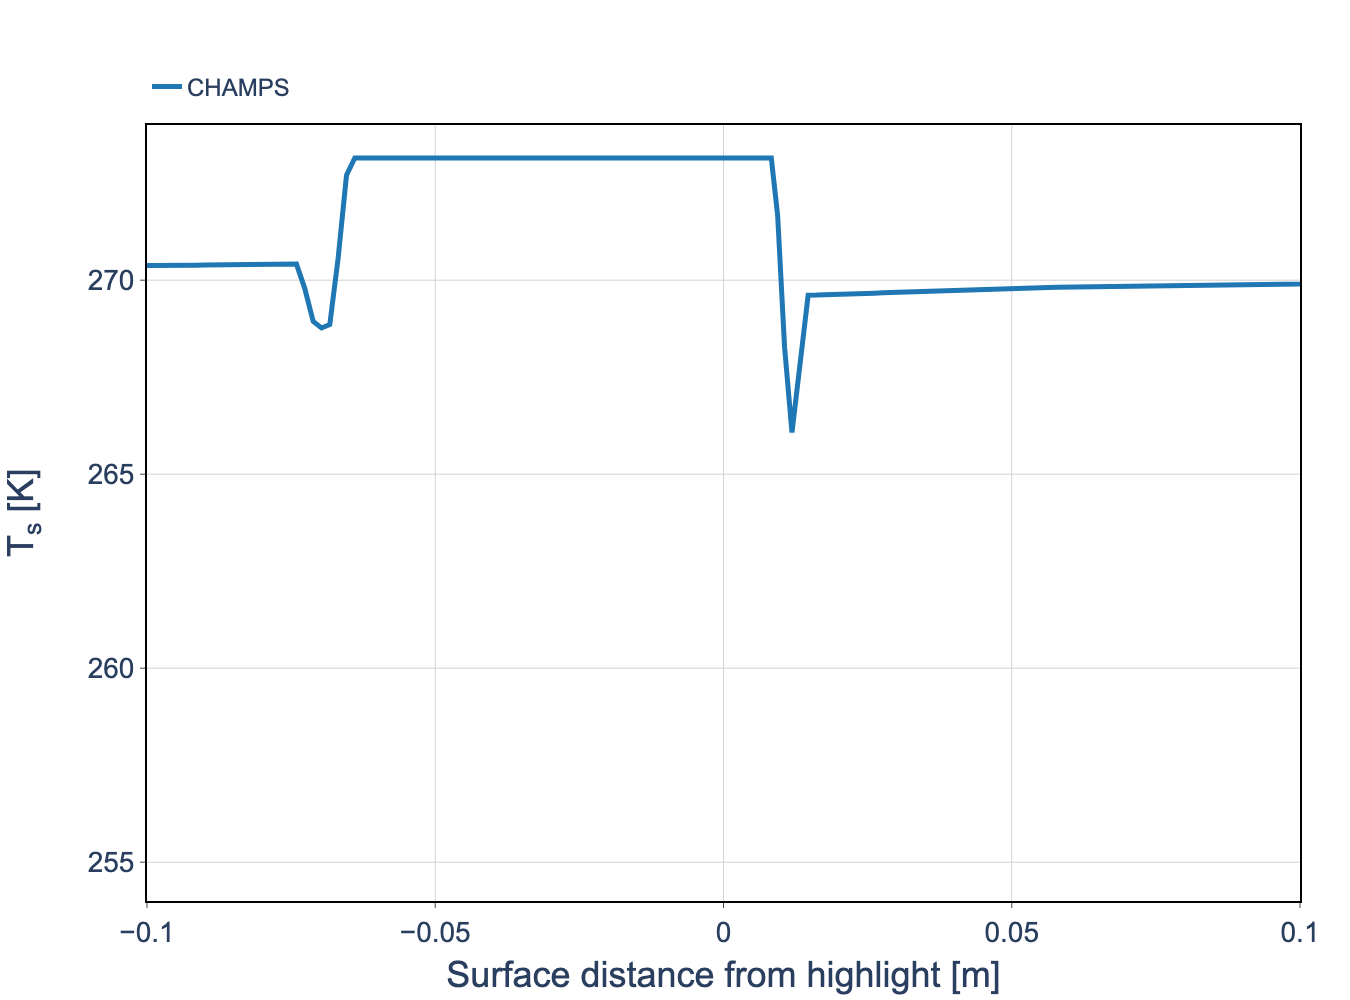
\includegraphics[
        width=\textwidth,
        trim={0cm 0cm 0cm 1.8cm},
        clip
    ]
    {FIGURES/NACA0012/SURF_TEMP_FF/tc_naca0012_ae3933_L1_surface_temperature_vs_s_slice_0p9144_all_roughness.png}
\end{column}

\end{columns}

\end{frame}


% ============================================================
% NACA0012 -- Upper-Horn Angle
% ============================================================

\begin{frame}{\small NACA0012 -- Upper-Horn Angle}
\scriptsize

\vspace{-0.15cm}

\begin{columns}[T,onlytextwidth]

% ------------------------------------------------------------
% AE3932
% ------------------------------------------------------------
\begin{column}{0.50\textwidth}
    \centering
    \textbf{AE3932}

    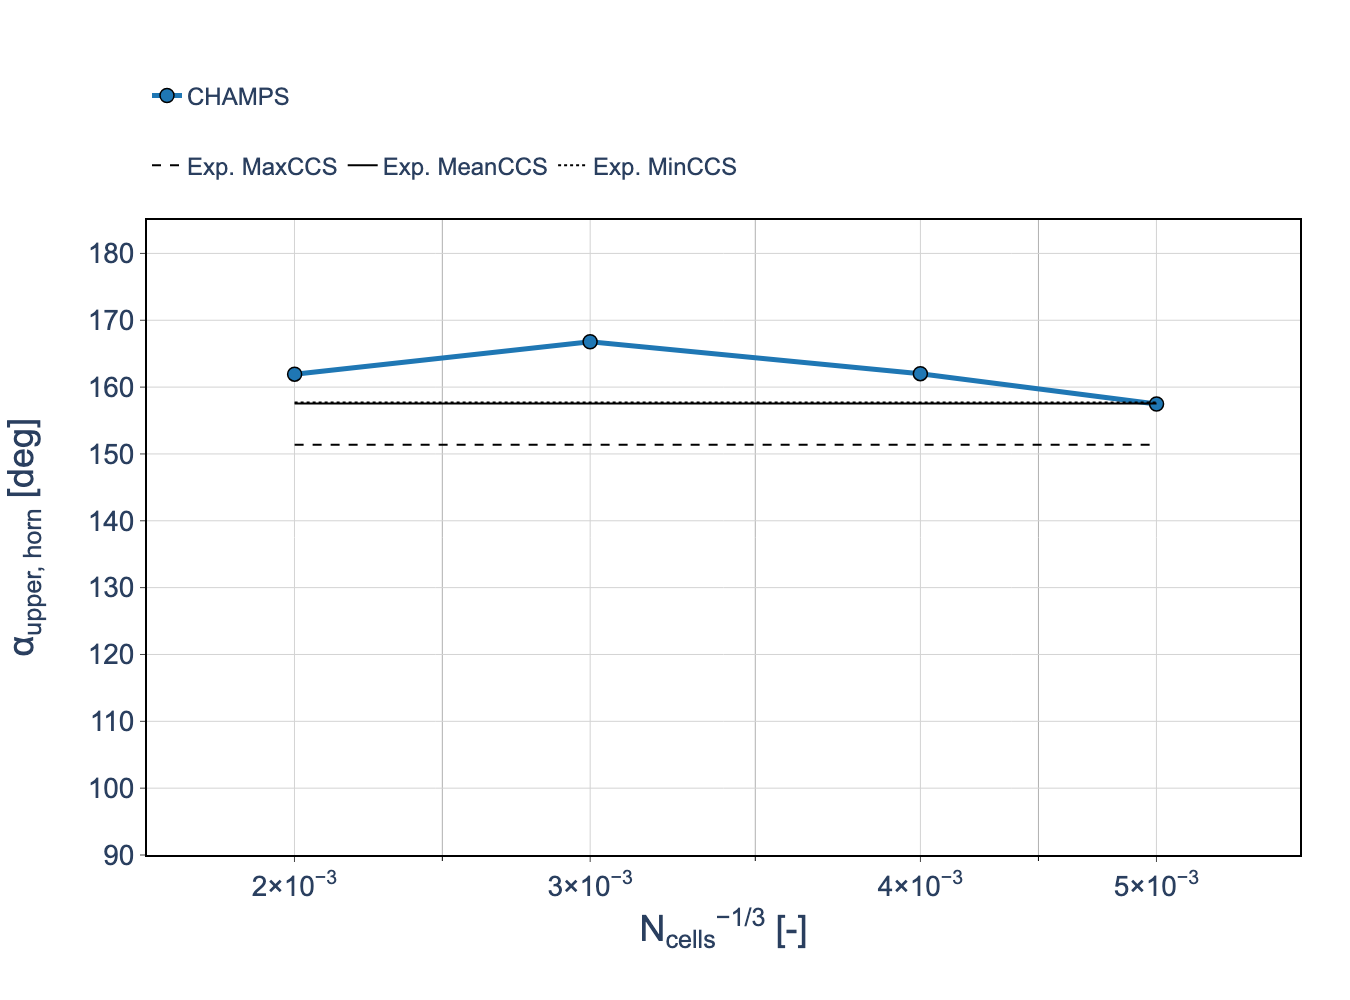
\includegraphics[
        width=\textwidth,
        trim={0cm 1cm 1cm 2.6cm},
        clip
    ]
    {FIGURES/NACA0012/ICE_ACCRETION/tc_naca0012_ae3932_upper_horn_angle_bins15.png}
\end{column}

% ------------------------------------------------------------
% AE3933
% ------------------------------------------------------------
\begin{column}{0.50\textwidth}
    \centering
    \textbf{AE3933}

    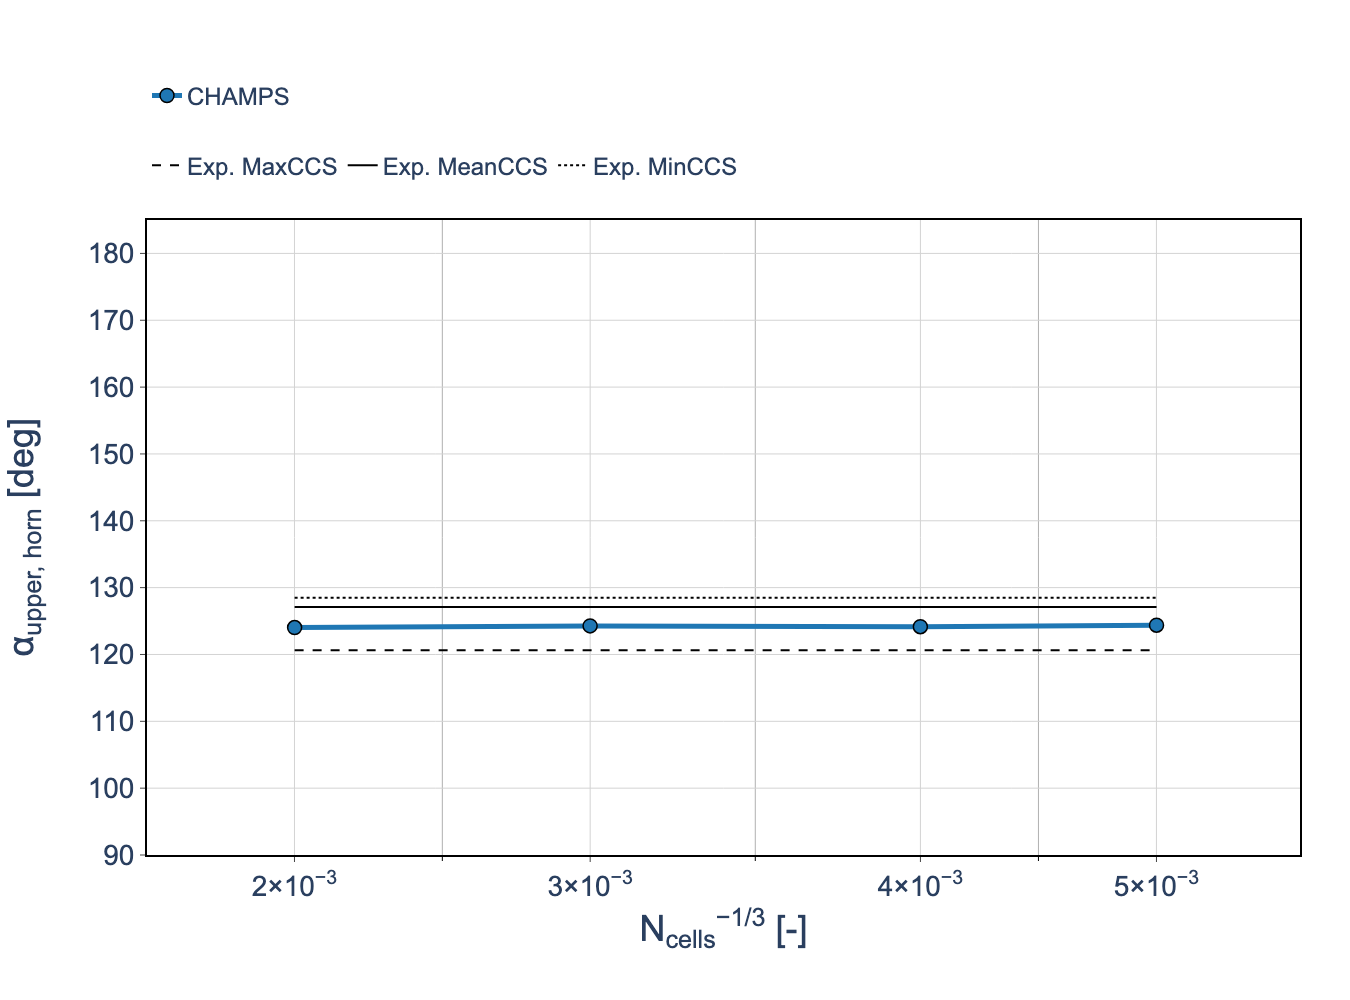
\includegraphics[
        width=\textwidth,
        trim={0cm 1cm 1cm 2.6cm},
        clip
    ]
    {FIGURES/NACA0012/ICE_ACCRETION/tc_naca0012_ae3933_upper_horn_angle_bins15.png}
\end{column}

\end{columns}

\vspace{-0.10cm}

\begin{block}{\scriptsize Assessment}
\begin{itemize}
    \item The predicted upper-horn angles agree well with experiment for both icing conditions.
    \item Droplet-bin refinement has negligible influence on the upper-horn angle (not shown due to limited variation).
    \item The substantial decrease in upper-horn angle from AE3932 to AE3933 is well captured.
\end{itemize}
\end{block}

\end{frame}

% ============================================================
% NACA0012 -- Multilayer Maximum Cross Sections
% ============================================================

\begin{frame}{\small NACA0012 -- Multilayer Maximum Cross Sections}
\scriptsize

\vspace{-0.15cm}

\begin{columns}[T,onlytextwidth]

% ------------------------------------------------------------
% AE3932
% ------------------------------------------------------------
\begin{column}{0.50\textwidth}
    \centering
    \textbf{AE3932}

    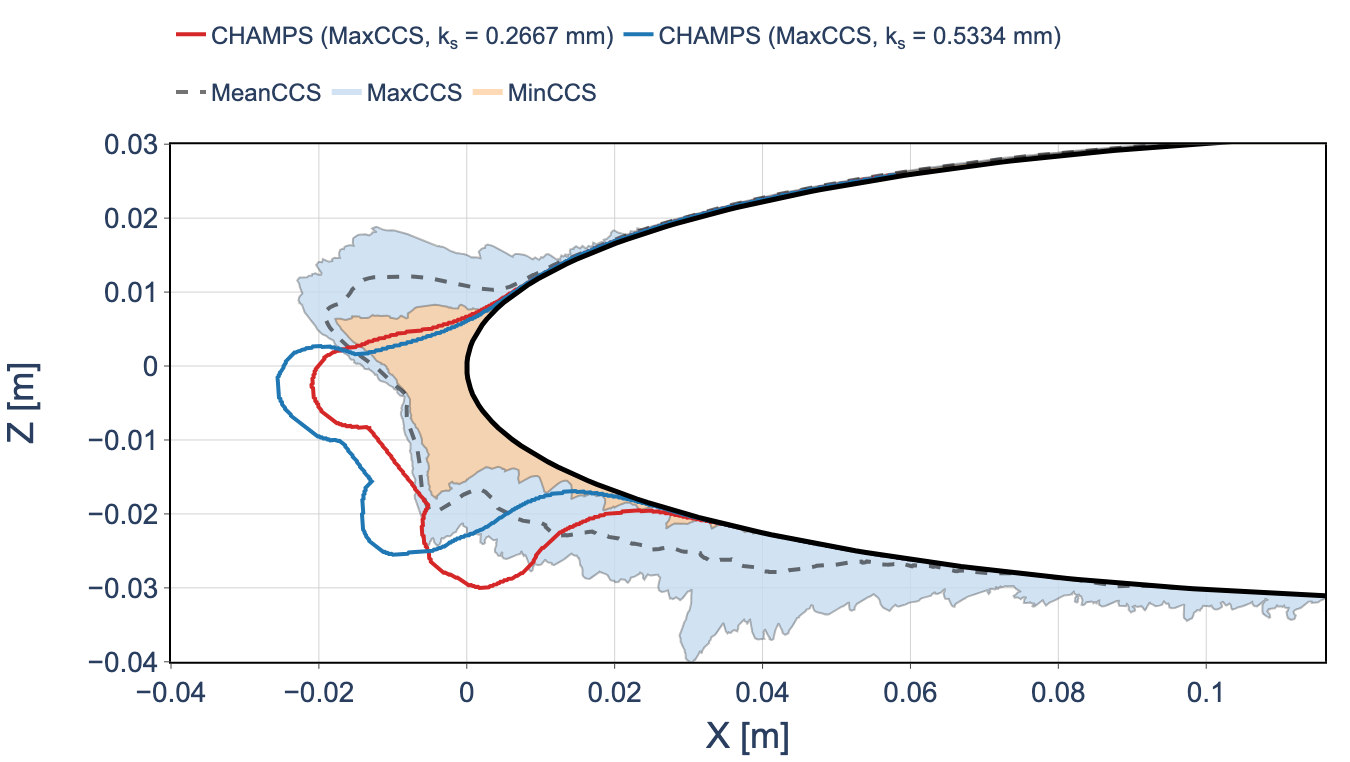
\includegraphics[
        width=\textwidth,
        trim={0cm 0cm 1cm 0.8cm},
        clip
    ]
    {FIGURES/NACA0012/ICE_SHAPES/tc_naca0012_ae3932_L1_multilayer_ice_shape_slice_0p9144_bins07_roughness_comparisons_MCCS.png}
\end{column}

% ------------------------------------------------------------
% AE3933
% ------------------------------------------------------------
\begin{column}{0.50\textwidth}
    \centering
    \textbf{AE3933}

    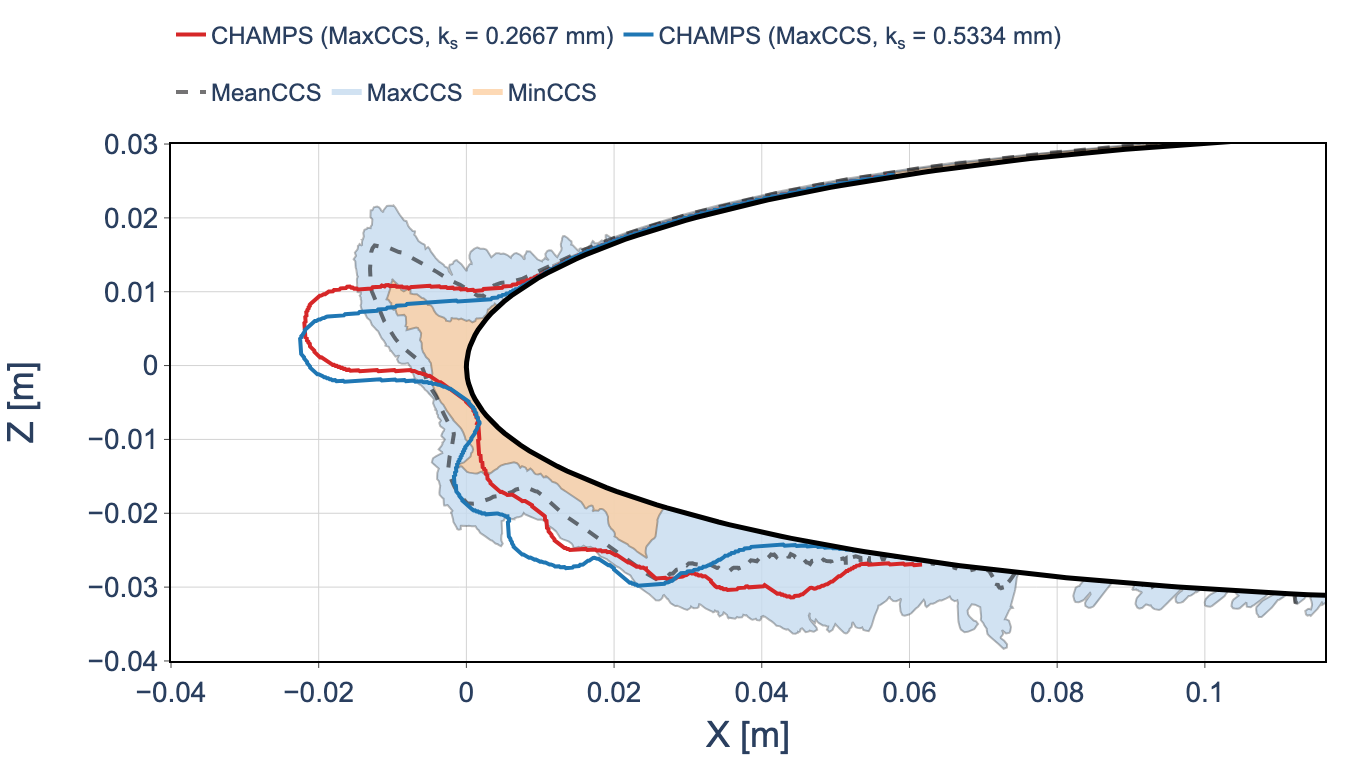
\includegraphics[
        width=\textwidth,
        trim={0cm 0cm 1cm 0.8cm},
        clip
    ]
    {FIGURES/NACA0012/ICE_SHAPES/tc_naca0012_ae3933_L1_multilayer_ice_shape_slice_0p9144_bins07_roughness_comparisons_MCCS.png}
\end{column}

\end{columns}

\vspace{-0.10cm}

\end{frame}

% ============================================================
% NACA0012 -- Effect of Surface-Normal Update
% ============================================================

\begin{frame}{\small NACA0012 -- Effect of Surface-Normal Update}
\scriptsize

\vspace{-0.15cm}

\begin{columns}[T,onlytextwidth]

% ------------------------------------------------------------
% AE3932
% ------------------------------------------------------------
\begin{column}{0.50\textwidth}
    \centering
    \textbf{AE3932}

    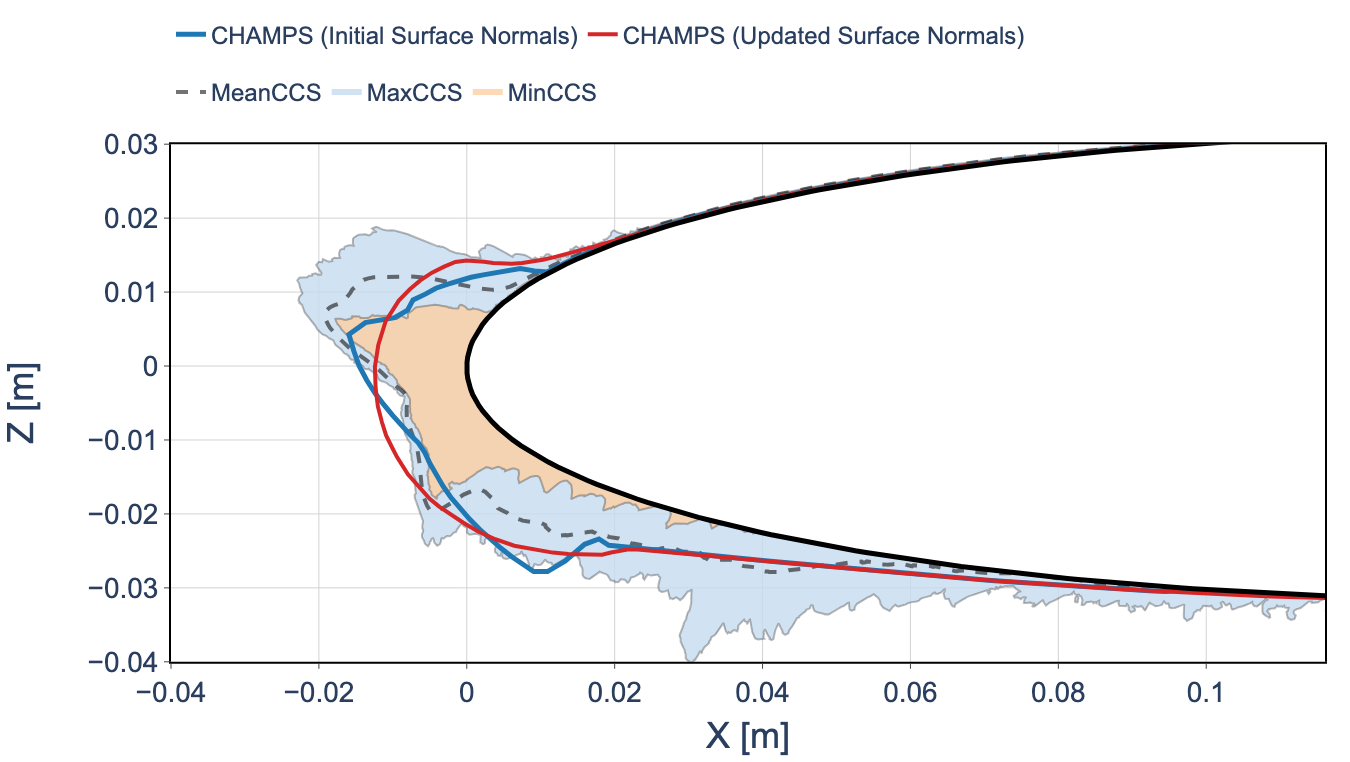
\includegraphics[
        width=\textwidth,
        trim={0cm 0cm 0cm 0.8cm},
        clip
    ]
    {FIGURES/NACA0012/ICE_SHAPES/tc_naca0012_ae3932_L1_single_layer_ice_shape_slice_0p9144_bins15_normals_comparison.png}
\end{column}

% ------------------------------------------------------------
% AE3933
% ------------------------------------------------------------
\begin{column}{0.50\textwidth}
    \centering
    \textbf{AE3933}

    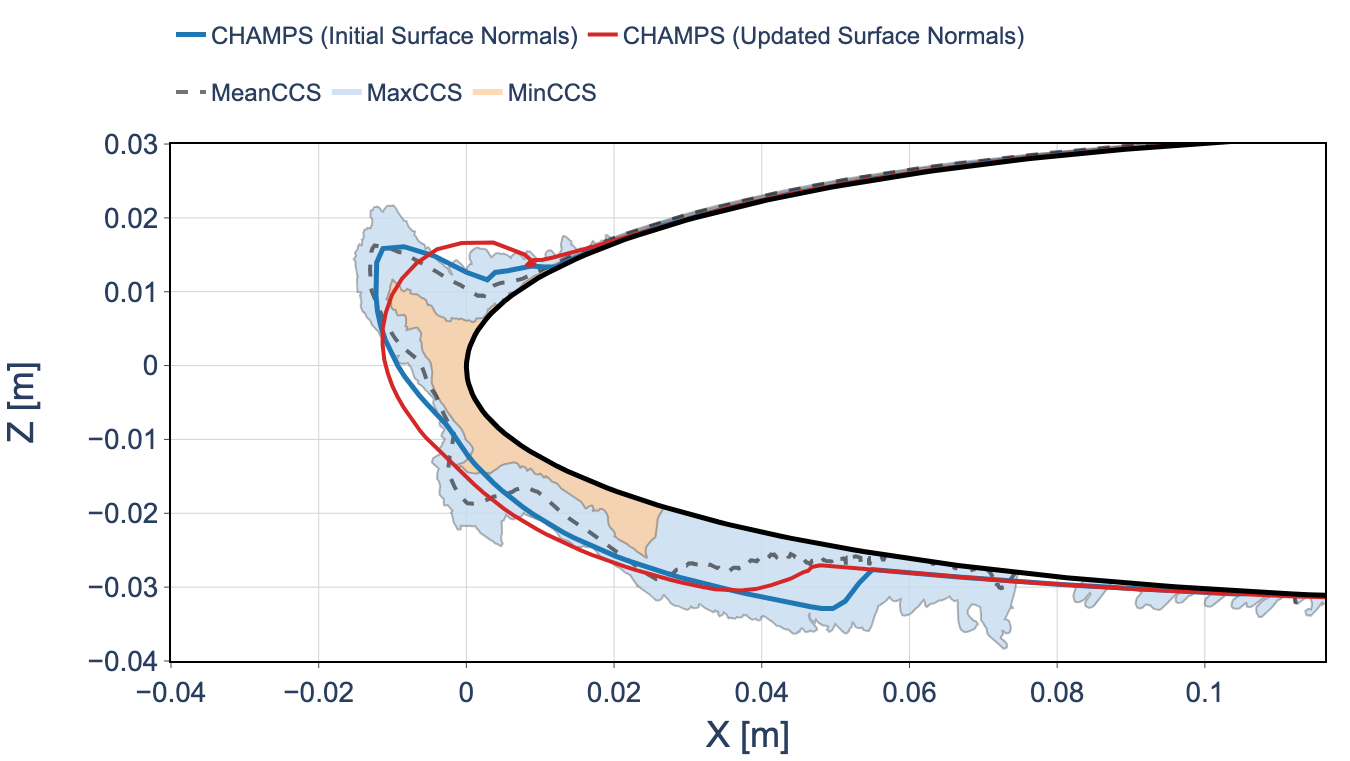
\includegraphics[
        width=\textwidth,
        trim={0cm 0cm 0cm 0.8cm},
        clip
    ]
    {FIGURES/NACA0012/ICE_SHAPES/tc_naca0012_ae3933_L1_single_layer_ice_shape_slice_0p9144_bins15_normals_comparison.png}
\end{column}

\end{columns}

\vspace{-0.10cm}

\begin{block}{\scriptsize Assessment}
\begin{itemize}
    \item Updating the surface normals while retaining the original surface accretion map produces a blunter horn and modifies its orientation.

    \item Retaining the initial normals provides better agreement with the experimental horn orientation for the present algebraic displacement.

    \item The updating of the surface accretion solution with the evolving normals was not considered in the present approach and will be investigated further.
\end{itemize}
\end{block}

\end{frame}



% ============================================================
% BACKUP -- ONERA M6 Convective Heat Transfer
% ============================================================

\begin{frame}{\small ONERA M6 -- Convective Heat-Transfer Coefficient}
\scriptsize

\vspace{-0.20cm}

\begin{columns}[T,onlytextwidth]

% ------------------------------------------------------------
% y = 0.10 m
% ------------------------------------------------------------
\begin{column}{0.33\textwidth}
    \centering
    \textbf{$y=0.10$ m}

    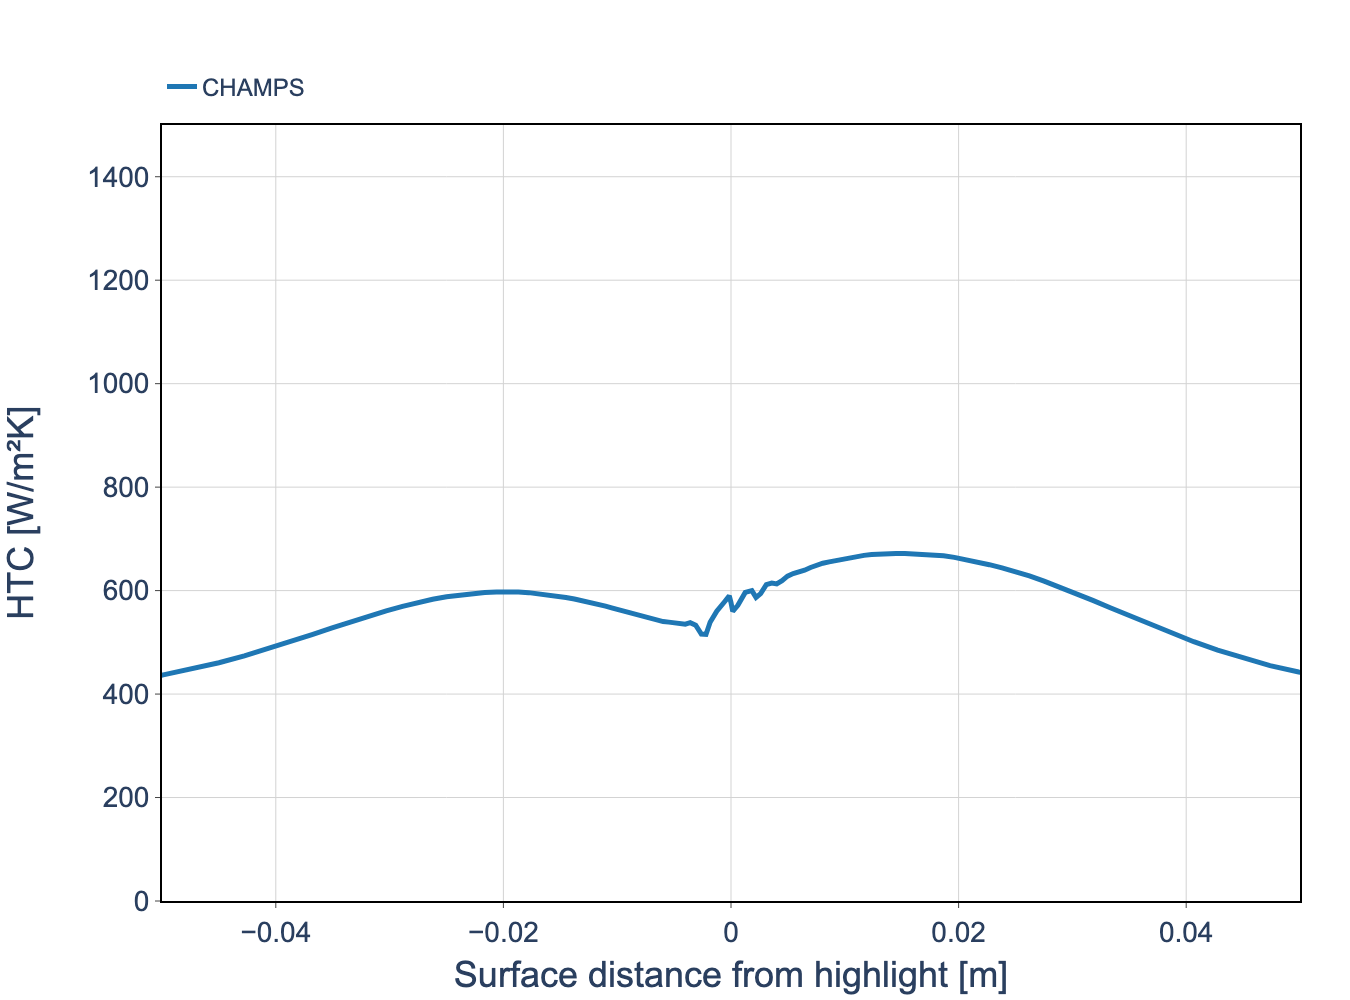
\includegraphics[
        width=\textwidth,
        trim={0cm 0cm 1cm 3.2cm},
        clip
    ]
    {FIGURES/ONERAM6/HTC/tc_oneram6_L1_htc_vs_s_slice_0p1_roughness_1mm.png}
\end{column}

% ------------------------------------------------------------
% y = 0.75 m
% ------------------------------------------------------------
\begin{column}{0.33\textwidth}
    \centering
    \textbf{$y=0.75$ m}

    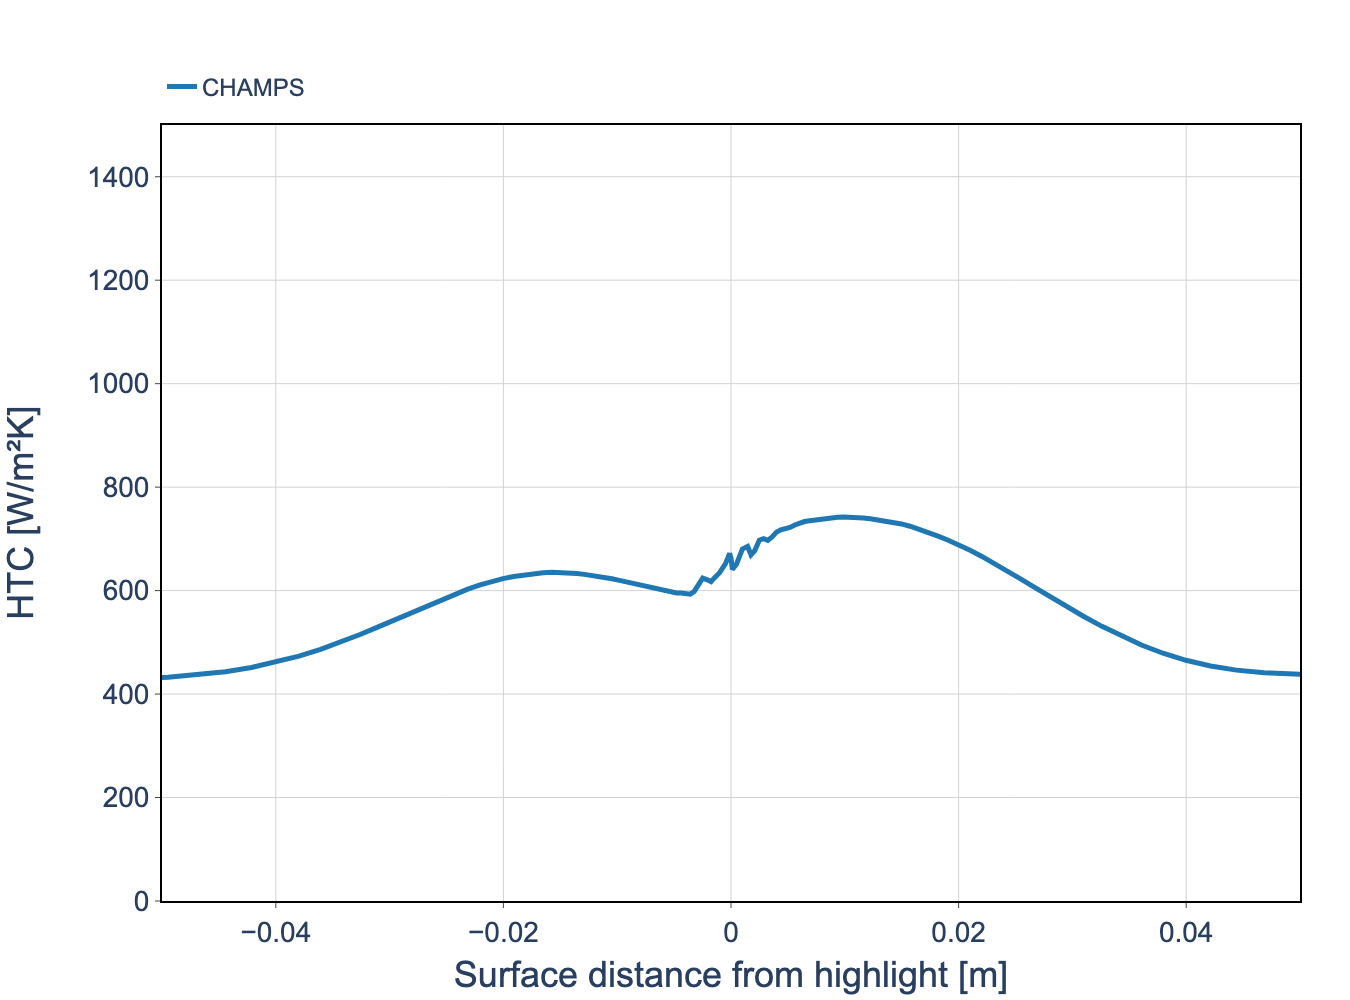
\includegraphics[
        width=\textwidth,
        trim={0cm 0cm 1cm 3.2cm},
        clip
    ]
    {FIGURES/ONERAM6/HTC/tc_oneram6_L1_htc_vs_s_slice_0p75_roughness_1mm.png}
\end{column}

% ------------------------------------------------------------
% y = 1.40 m
% ------------------------------------------------------------
\begin{column}{0.33\textwidth}
    \centering
    \textbf{$y=1.40$ m}

    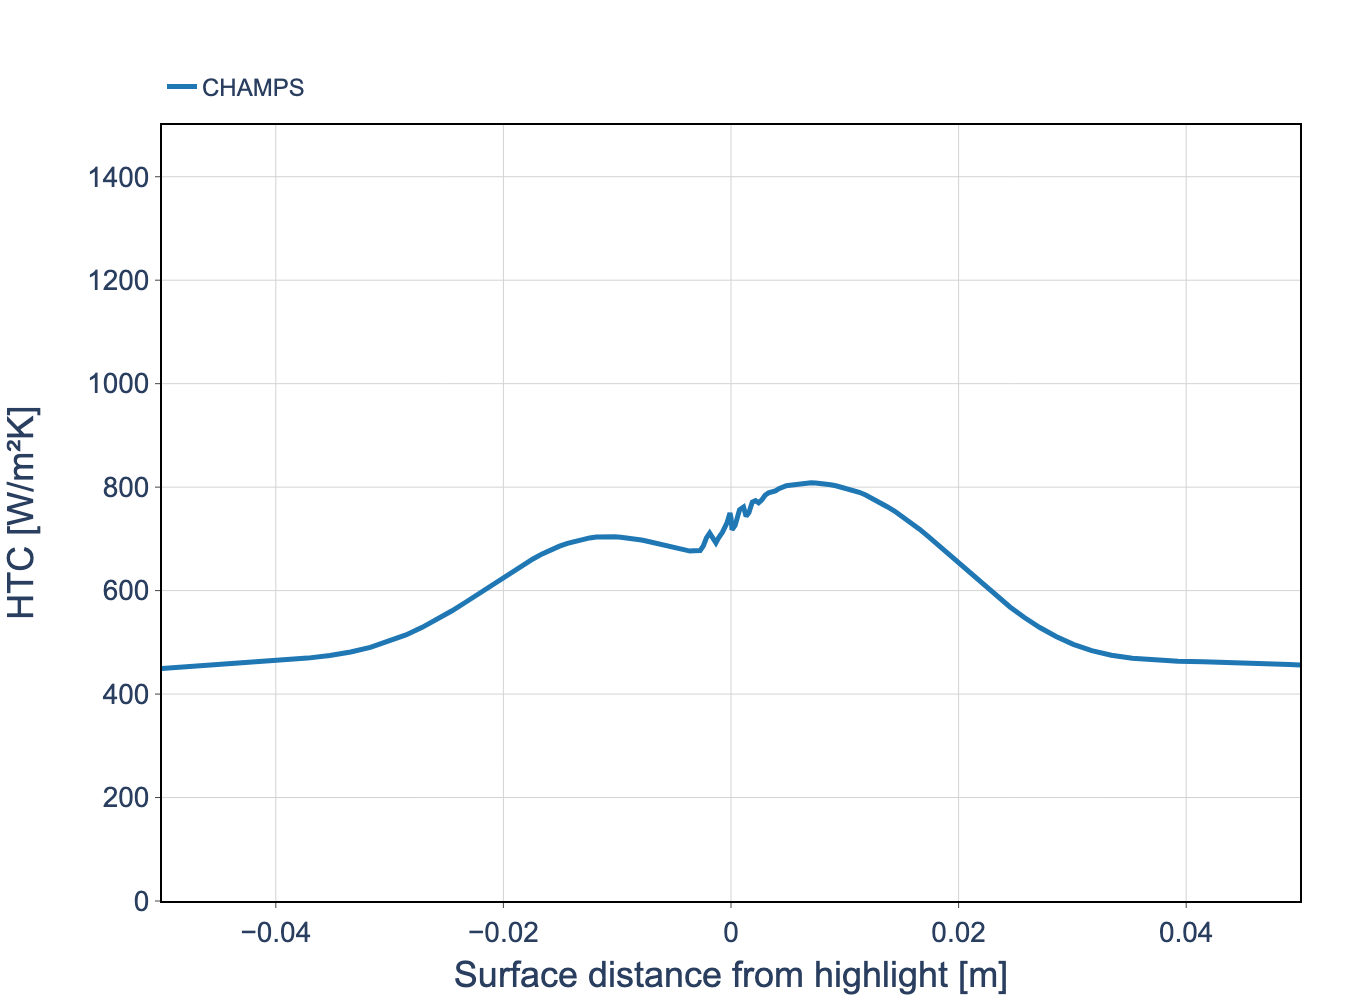
\includegraphics[
        width=\textwidth,
        trim={0cm 0cm 1cm 3.2cm},
        clip
    ]
    {FIGURES/ONERAM6/HTC/tc_oneram6_L1_htc_vs_s_slice_1p4_roughness_1mm.png}
\end{column}

\end{columns}

\end{frame}

% ============================================================
% BACKUP -- ONERA M6 Thermodynamics
% ============================================================

\begin{frame}{\small ONERA M6 -- Surface Thermodynamics ($y=0.75$ m)}
\scriptsize

\vspace{-0.20cm}

\begin{columns}[T,onlytextwidth]

% ------------------------------------------------------------
% Surface Temperature
% ------------------------------------------------------------
\begin{column}{0.50\textwidth}
    \centering
    \textbf{Surface Temperature}

    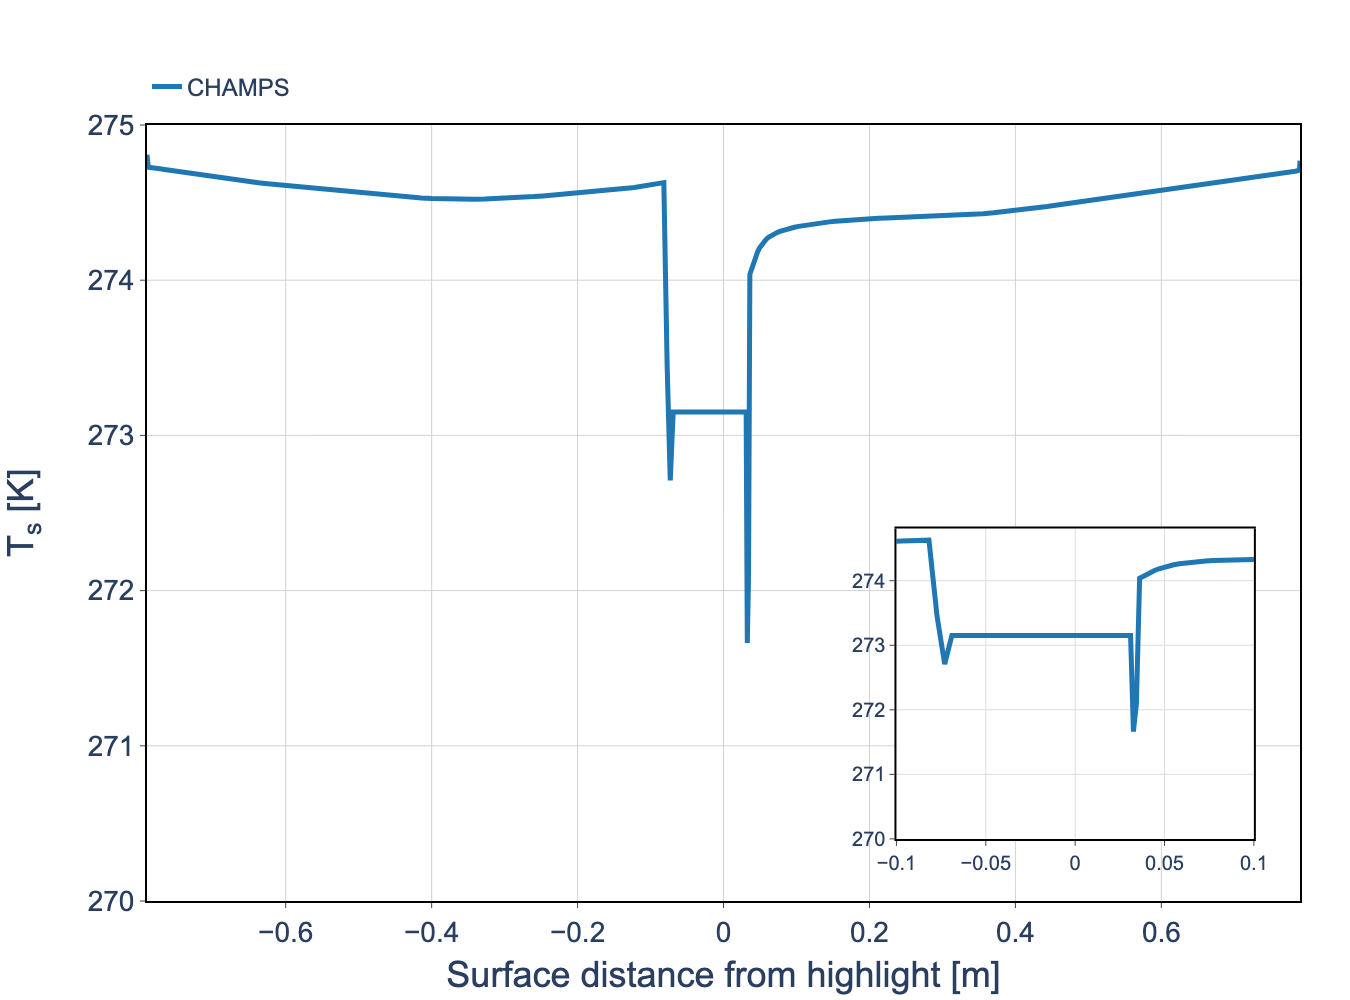
\includegraphics[
        width=\textwidth,
        trim={0cm 0cm 1cm 3.2cm},
        clip
    ]
    {FIGURES/ONERAM6/SURF_TEMP_FF/tc_oneram6_L1_surface_temperature_vs_s_slice_0p75_roughness_1mm.png}
\end{column}

% ------------------------------------------------------------
% Freezing Fraction
% ------------------------------------------------------------
\begin{column}{0.50\textwidth}
    \centering
    \textbf{Freezing Fraction}

    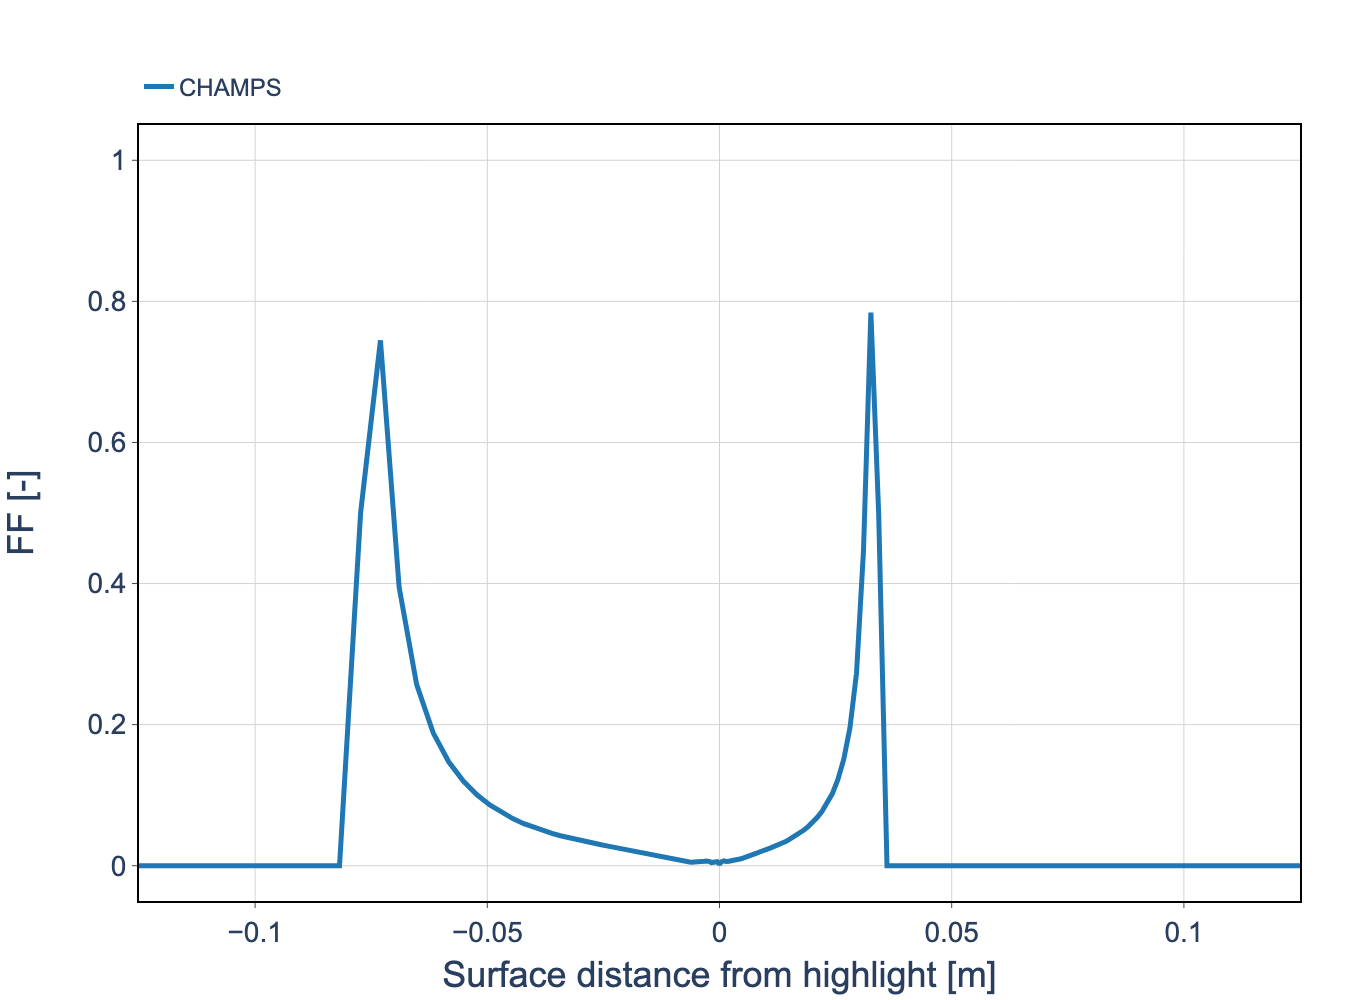
\includegraphics[
        width=\textwidth,
        trim={0cm 0cm 1cm 3.2cm},
        clip
    ]
    {FIGURES/ONERAM6/SURF_TEMP_FF/tc_oneram6_L1_freezing_fraction_vs_s_slice_0p75_roughness_1mm.png}
\end{column}

\end{columns}

\end{frame}

% ============================================================
% BACKUP -- ONERA M6 -- Surface-Normal Update
% ============================================================

\begin{frame}{\small ONERA M6 -- Effect of Surface-Normal Update}
\scriptsize

\vspace{-0.20cm}

\begin{columns}[T,onlytextwidth]

% ------------------------------------------------------------
% y = 0.10 m
% ------------------------------------------------------------
\begin{column}{0.33\textwidth}
    \centering
    \textbf{$y=0.10$ m}

    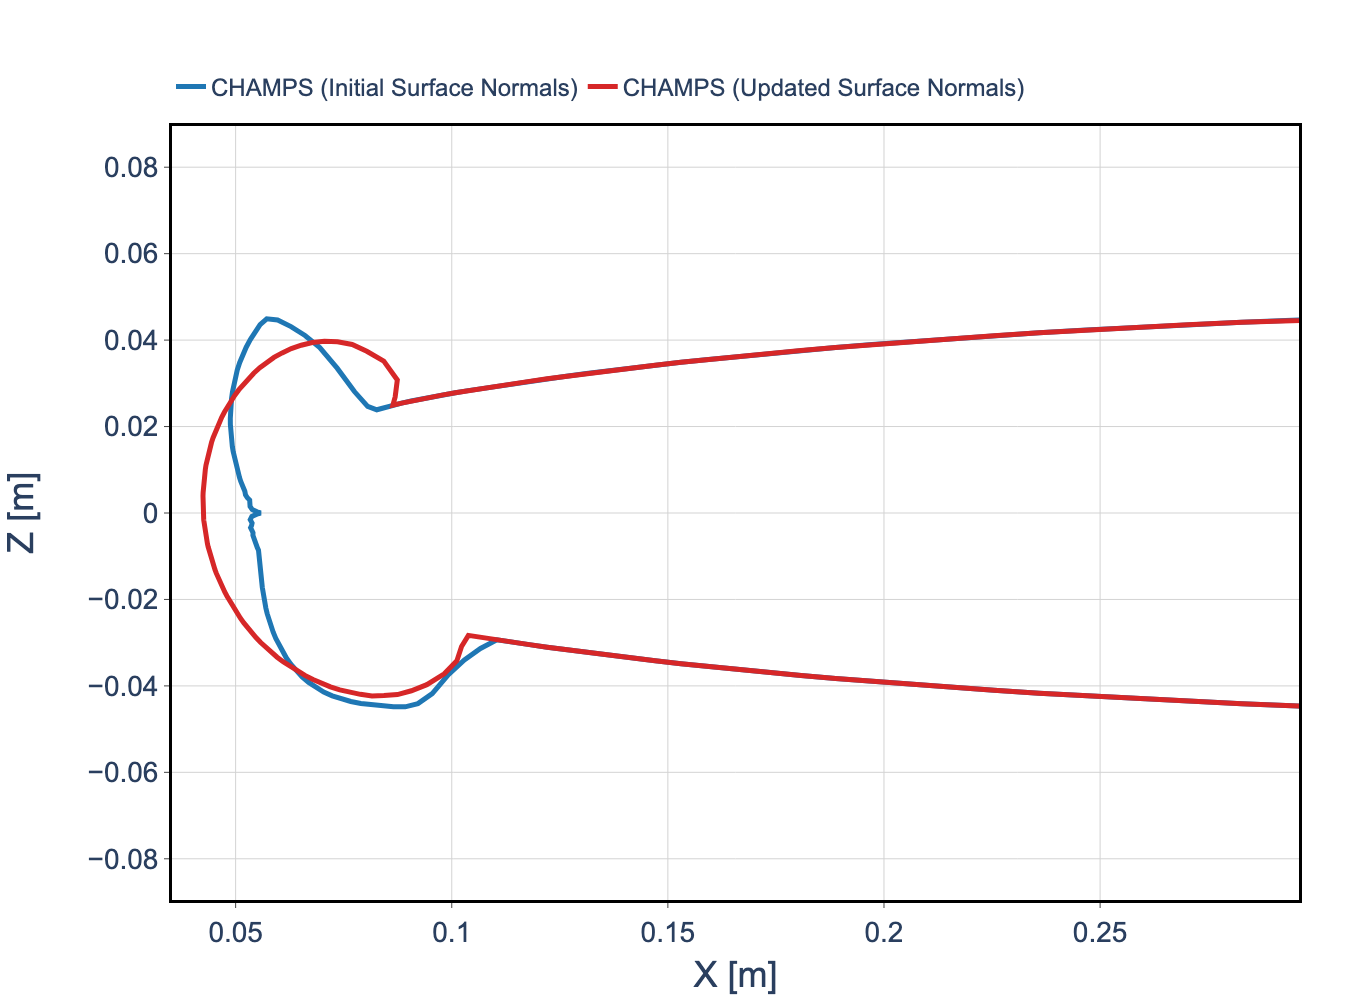
\includegraphics[
        width=\textwidth,
        trim={0cm 0cm 0cm 2.5cm},
        clip
    ]
    {FIGURES/ONERAM6/ICE_SHAPES/tc_oneram6_L1_single_layer_ice_shape_slice_0p1_bins15_normals_comparison.png}
\end{column}

% ------------------------------------------------------------
% y = 0.75 m
% ------------------------------------------------------------
\begin{column}{0.33\textwidth}
    \centering
    \textbf{$y=0.75$ m}

    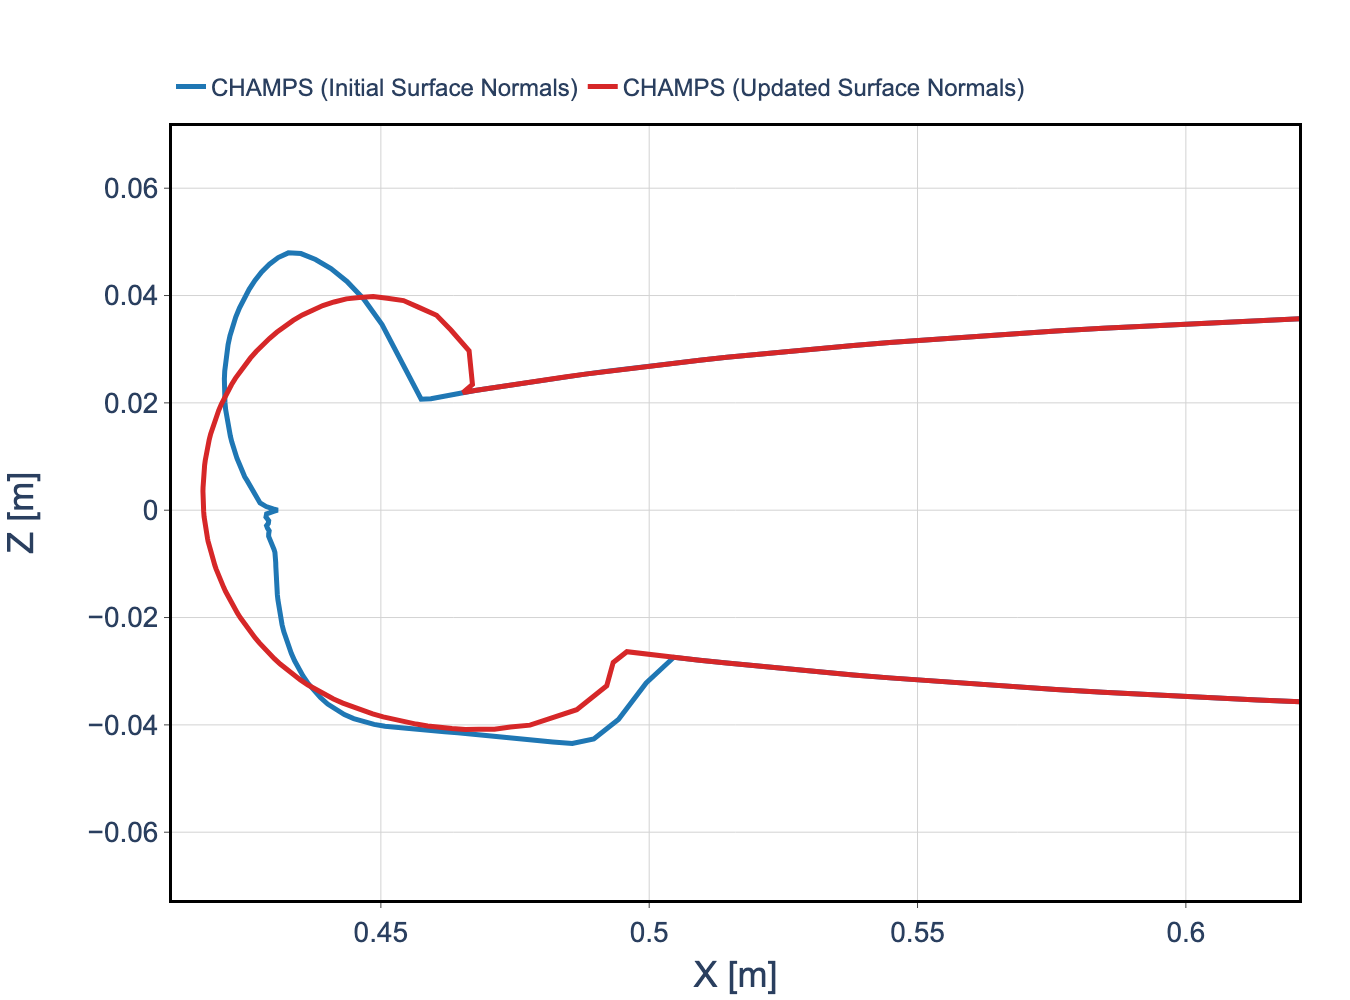
\includegraphics[
        width=\textwidth,
        trim={0cm 0cm 0cm 2.5cm},
        clip
    ]
    {FIGURES/ONERAM6/ICE_SHAPES/tc_oneram6_L1_single_layer_ice_shape_slice_0p75_bins15_normals_comparison.png}
\end{column}

% ------------------------------------------------------------
% y = 1.40 m
% ------------------------------------------------------------
\begin{column}{0.33\textwidth}
    \centering
    \textbf{$y=1.40$ m}

    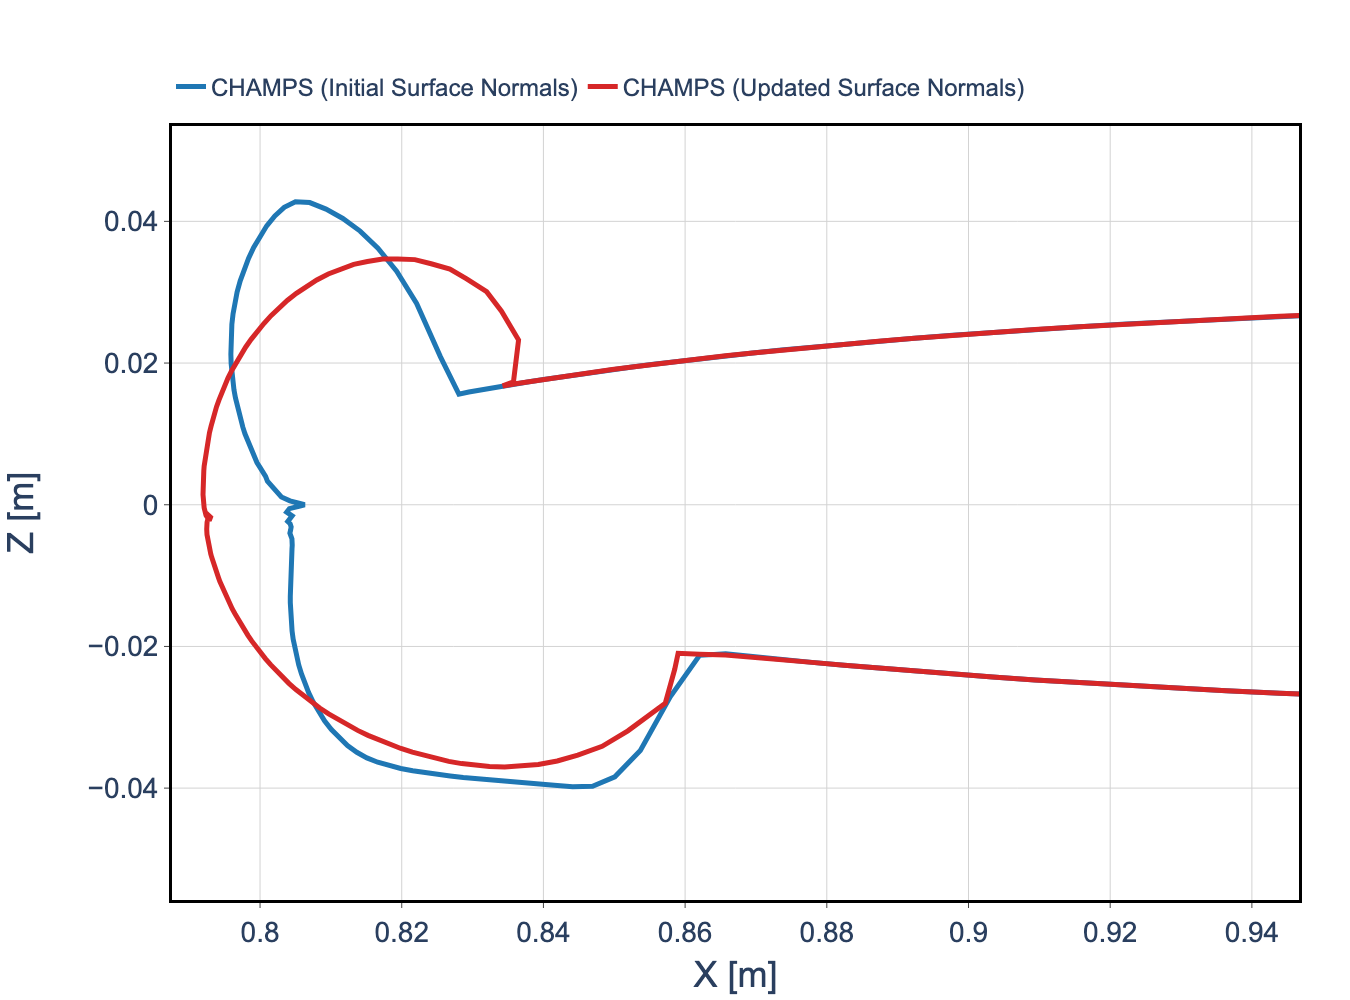
\includegraphics[
        width=\textwidth,
        trim={0cm 0cm 0cm 2.5cm},
        clip
    ]
    {FIGURES/ONERAM6/ICE_SHAPES/tc_oneram6_L1_single_layer_ice_shape_slice_1p4_bins15_normals_comparison.png}
\end{column}

\end{columns}

\end{frame}


% ============================================================
% CHAMPS -- LEVEL-SET GEOMETRY EVOLUTION
% ============================================================

\begin{frame}[c]{\small CHAMPS -- Multilayer Level-Set Evolution}
\scriptsize

\centering

% ============================================================
% STEP 1 -- GENERATE LEVEL-SET MESH
% ============================================================
\only<1>{

% Framework -- Step 1 highlighted
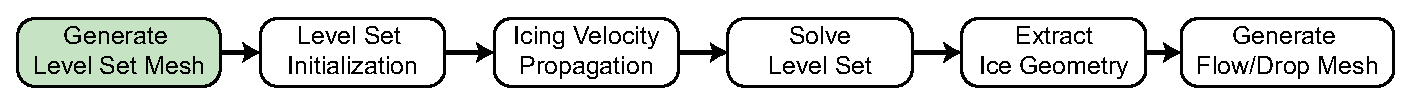
\includegraphics[
    width=0.95\textwidth
]{FIGURES/LS_FRAMEWORK/LS_STEP_1.eps}

\vspace{0.20cm}

\begin{block}{\scriptsize Generate Level-Set Mesh}
A dedicated level-set mesh is generated to avoid the restrictive
time-step requirements of the highly refined near-wall RANS mesh.
The mesh is adapted to encompass the expected ice-thickness extent.
\end{block}

\vspace{0.15cm}

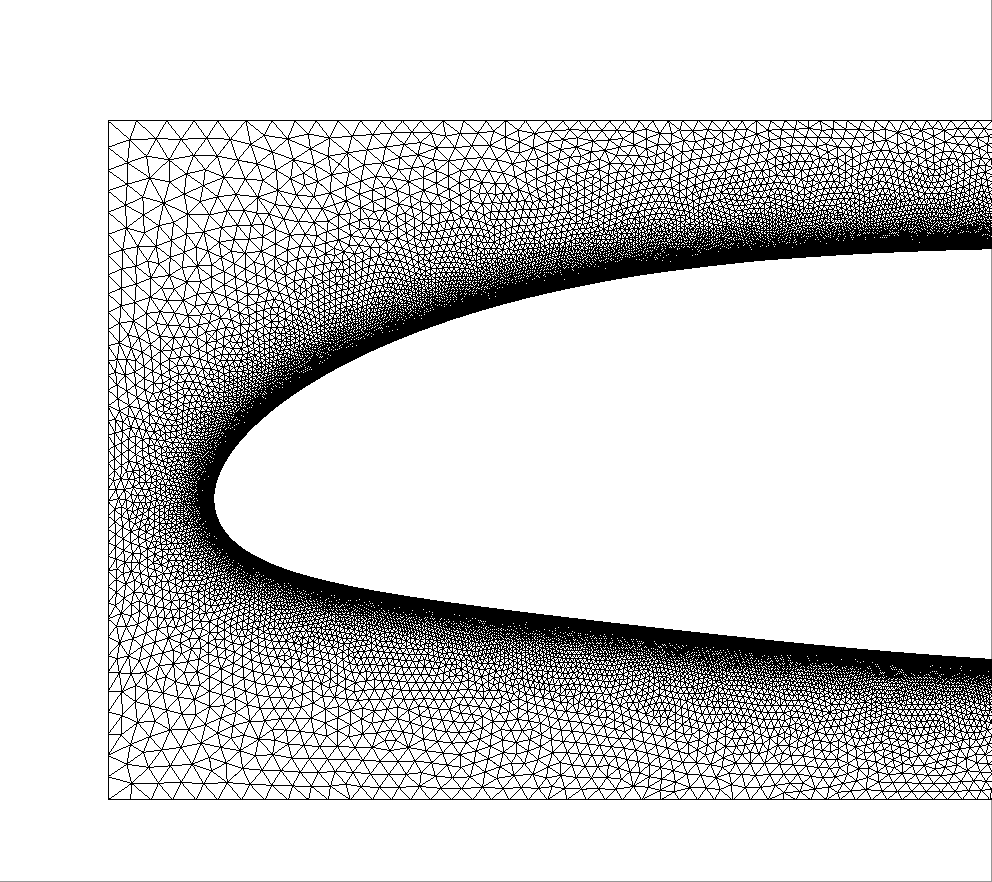
\includegraphics[
    width=0.4\textwidth,
    trim={0cm 0.1cm 3cm 3cm},
    clip
]{FIGURES/LS_FRAMEWORK/MESH_ADAPTATION.png}

}

% ============================================================
% STEP 2 -- LEVEL-SET INITIALIZATION
% ============================================================
\only<2>{

% Framework -- Step 2 highlighted
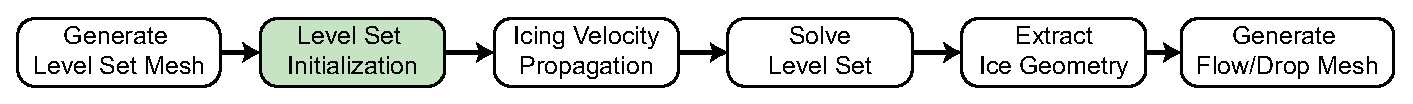
\includegraphics[
    width=0.95\textwidth
]{FIGURES/LS_FRAMEWORK/LS_STEP_2.eps}

\vspace{0.20cm}

\begin{block}{\scriptsize Level-Set Initialization}
The level-set field is initialized as a signed-distance function
from the current ice--air interface using an \textbf{Eikonal-based
wall-distance method} or an equivalent wall-distance technique.
\end{block}

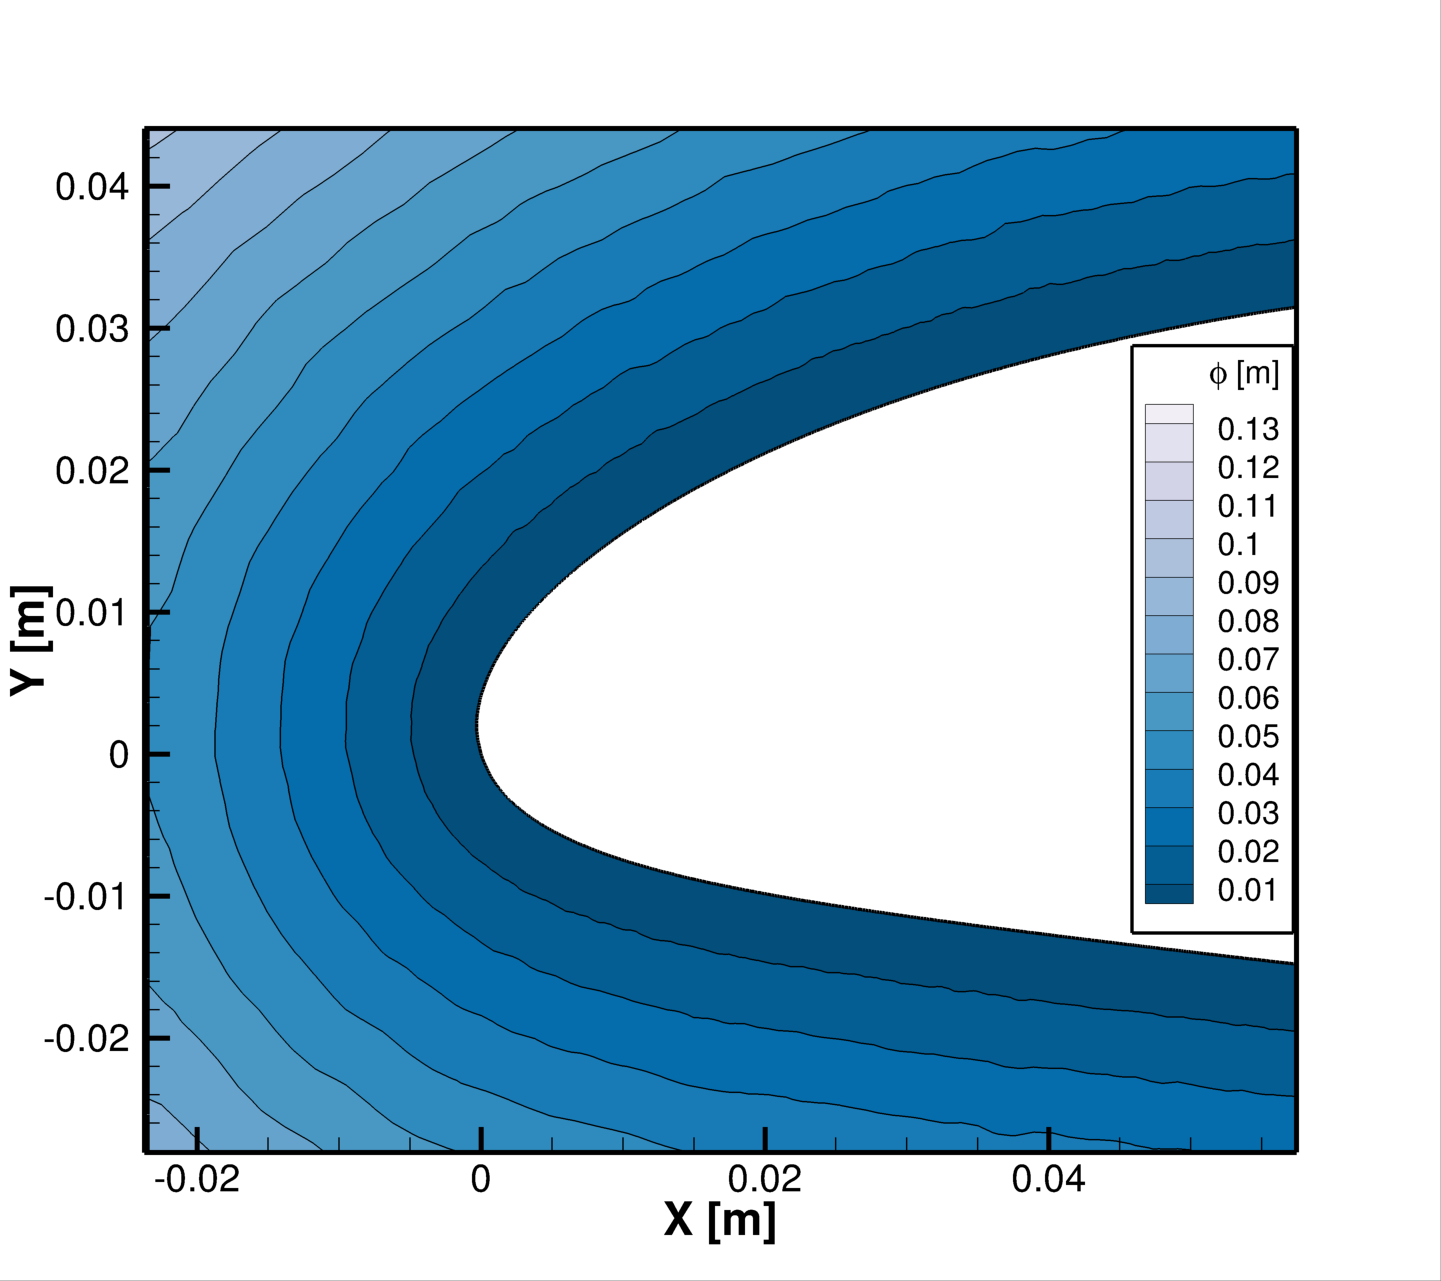
\includegraphics[
    width=0.35\textwidth,
    trim={0cm 0.1cm 3cm 3cm},
    clip
]{FIGURES/LS_FRAMEWORK/EIKONAL.png}

}

% ============================================================
% STEP 3 -- ICING VELOCITY PROPAGATION
% ============================================================
\only<3>{

% Framework -- Step 3 highlighted
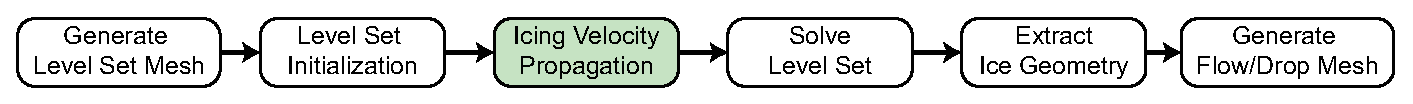
\includegraphics[
    width=0.95\textwidth
]{FIGURES/LS_FRAMEWORK/LS_STEP_3.eps}

\vspace{0.20cm}

\begin{block}{\scriptsize Icing Velocity Propagation}
The interface velocity magnitude,
$V_{\mathrm{ice}} = h_{\mathrm{ice}}/\Delta t_{\mathrm{layer}}$,
is propagated from the ice--air interface into the level-set domain.
The interface velocity is then constructed using the level-set normal:
\[
\boldsymbol{V}
=
V_{\mathrm{ice}}\,\boldsymbol{n}_{\phi}.
\]
\end{block}


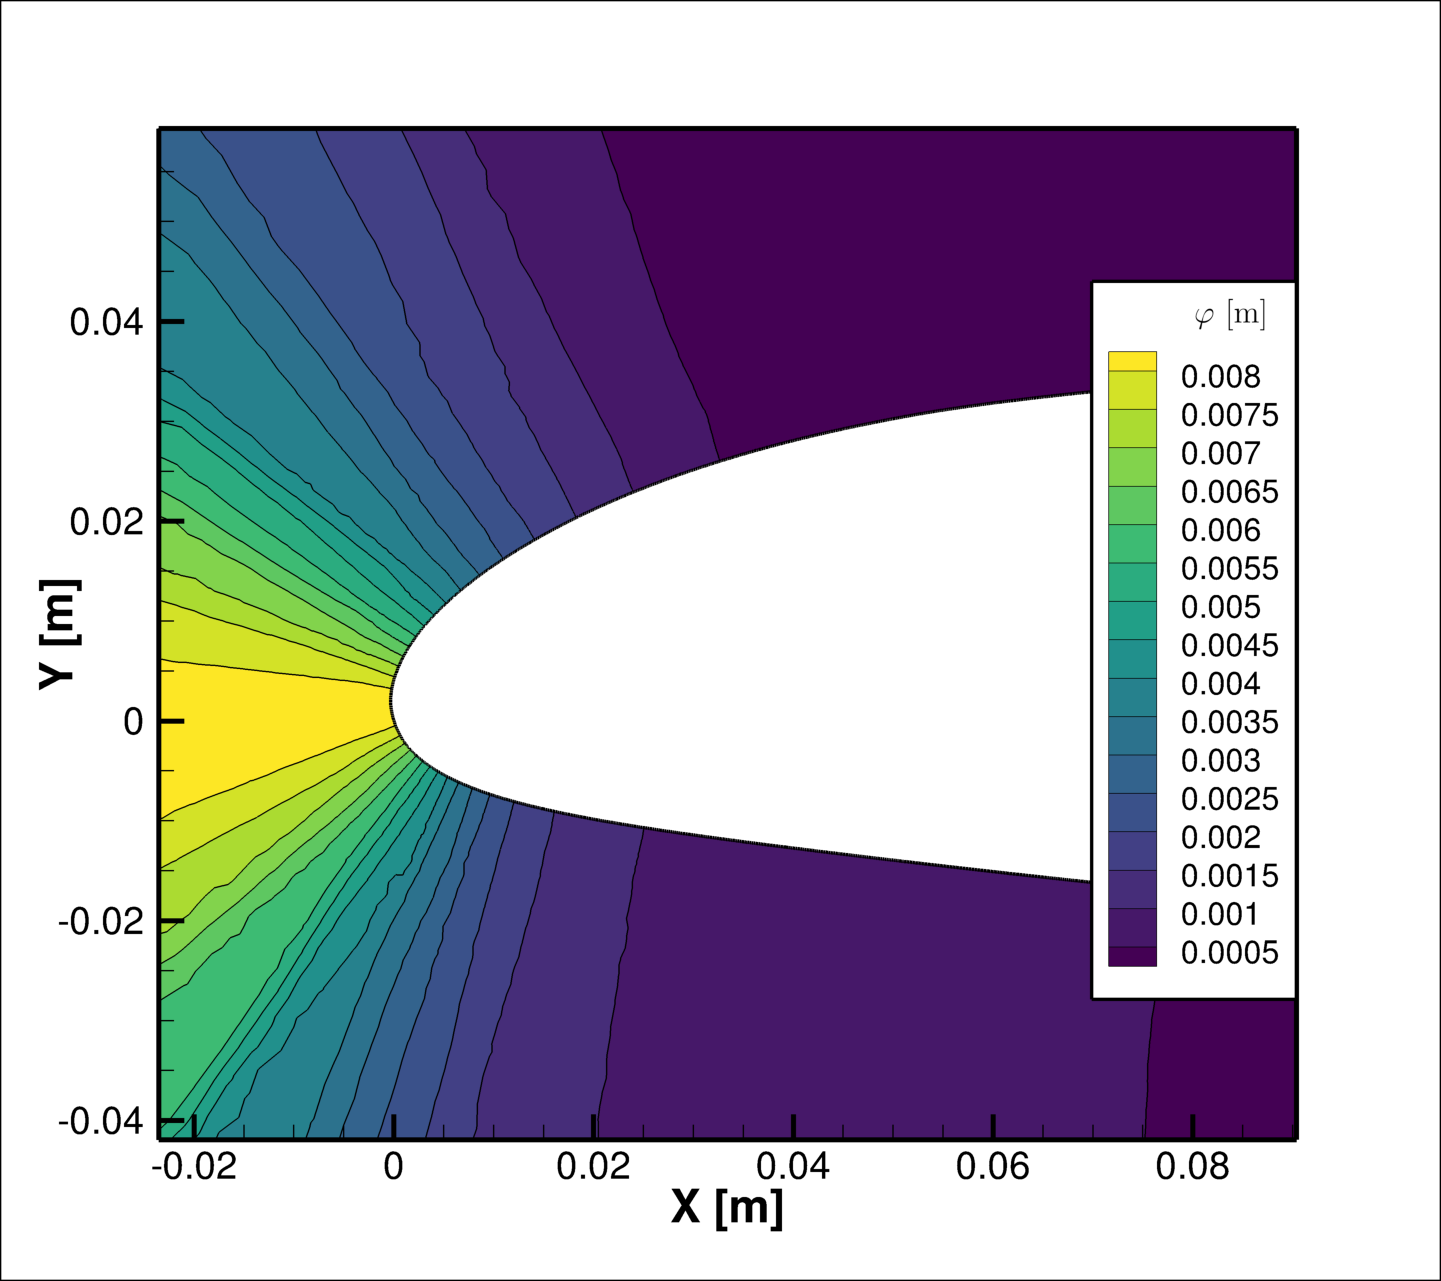
\includegraphics[
    width=0.35\textwidth,
    trim={0.1cm 0.1cm 3cm 3cm},
    clip
]{FIGURES/LS_FRAMEWORK/PROPAGATION.png}

}

% ============================================================
% STEP 4 -- SOLVE LEVEL SET
% ============================================================
\only<4>{

% Framework -- Solve Level Set highlighted
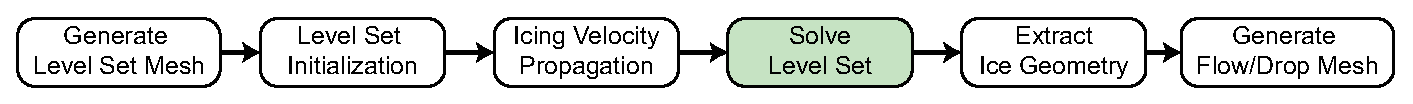
\includegraphics[
    width=0.95\textwidth
]{FIGURES/LS_FRAMEWORK/LS_STEP_4.eps}

\vspace{0.20cm}

\begin{block}{\scriptsize Solve Level Set -- Rosenbrock--Wanner (ROW) Scheme}

\begin{itemize}

    \item The level-set transport equation is advanced using a
    \textbf{two-stage Rosenbrock--Wanner (ROW) semi-implicit scheme}:

    \vspace{-0.10cm}

    \[
    \phi^{n+1}
    =
    \phi^n+\sum_{j=1}^{s}m_jS_j,
    \qquad
    \left(
    \frac{\boldsymbol{I}}{\gamma\Delta t}
    +\boldsymbol{J}
    \right)^n S_i
    =
    -R\left(
    \phi^n+\sum_{j=1}^{i-1}a_{ij}S_j
    \right).
    \]

    \vspace{-0.10cm}

    \item The ROW scheme has demonstrated
    \textbf{excellent performance for flow time integration in CHAMPS},
    providing improved stability and allowing larger time steps;
    it was therefore adopted for the level-set equation.

    \item At each ROW stage, a \textbf{linear system} is solved iteratively
    using \textbf{GMRES}:
    \[
    \underbrace{
    \left(
    \frac{\boldsymbol{I}}{\gamma\Delta t}
    +\boldsymbol{J}
    \right)^n}_{\boldsymbol{A}}
    S_i
    =
    \underbrace{
    -R\left(
    \phi^n+\sum_{j=1}^{i-1}a_{ij}S_j
    \right)}_{\boldsymbol{b}_i}.
    \]

\end{itemize}

\vspace{-0.10cm}

{\tiny
\textbf{*}
$\phi^n$: level-set solution;
$S_i$: stage increment;
$s$: number of ROW stages;
$m_j$, $a_{ij}$: ROW coefficients;
$\gamma$: ROW parameter;
$\Delta t$: time step;
$\boldsymbol{I}$: identity matrix;
$R(\phi)$: spatial residual;
$\boldsymbol{J}=\partial R/\partial\phi$: residual Jacobian.
}

\end{block}

}

% ============================================================
% STEP 5 -- EXTRACT ICE GEOMETRY
% ============================================================
\only<5>{

% Framework -- Step 5 highlighted
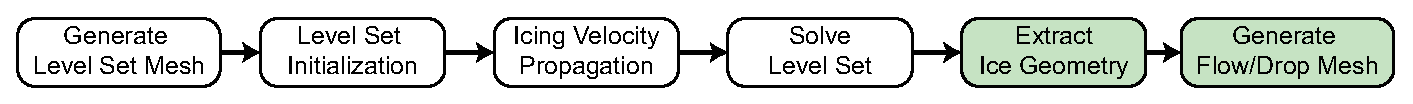
\includegraphics[
    width=0.95\textwidth
]{FIGURES/LS_FRAMEWORK/LS_STEP_5.eps}

\vspace{0.20cm}

\begin{block}{\scriptsize Extract Ice Geometry \& Generate Volume Mesh}
The updated ice surface is extracted from the volumetric level-set
solution as the $\phi=0$ isosurface using \textbf{MMG}. A new
\textbf{volume mesh} is then generated around the updated ice geometry
using \textbf{Pointwise Python scripts}.
\end{block}

\vspace{0.15cm}

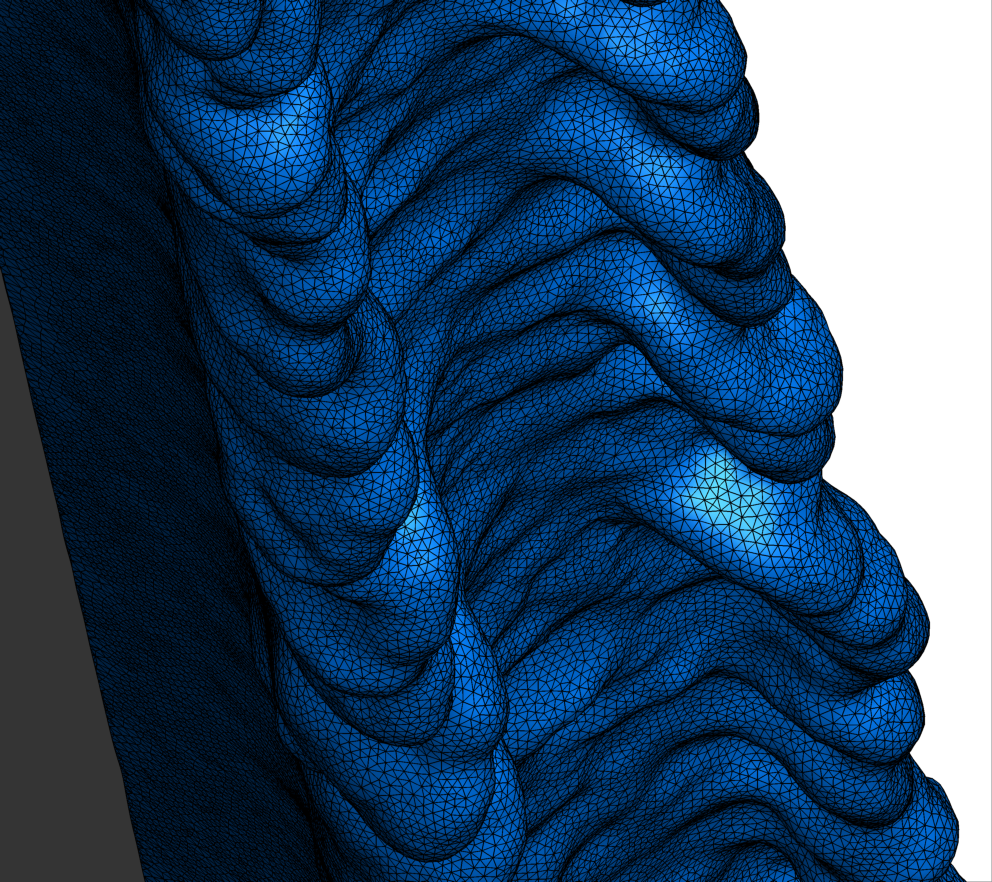
\includegraphics[
    width=0.4\textwidth
]{FIGURES/LS_FRAMEWORK/CLIPPED_ICE_SHAPE_CASE_362_3.png}

}

\end{frame}
